\chapter{Algoritamske paradigme}

\textit{Programske paradigme} predstavljaju različite pristupe ili stilove  programiranja koji definišu način na koji programeri dizajniraju, strukturiraju i organizuju  svoj k\^od za rješavanje problema. Postoji nekoliko programskih paradigmi, a svaka od njih zahtjeva  drugačiji način razmišljanja o problemima i rješenjima programiranja.

Neke od najčešćih programskih paradigmi su date u nastavku. 

\begin{itemize}
	\item \textit{Imperativno programiranje}: Ova paradigma uključuje %upotrebu naredbi koji mijenjaju stanje programa, a sastoji se od
	 eksplicitni slijed naredbi koje računar izvršava određenim redoslijedom.
	\item \textit{Funkcijsko programiranje}: Ova paradigma se fokusira na korištenje funkcija za rješavanje problema.  %, sa naglaskom na nepromjenjivosti i izbjegavanju nuspojava.
	\item \textit{Logičko programiranje}: Ova paradigma uključuje programiranje zasnovano na logici i zaključivanju. Posebno je koristan za probleme koji uključuju pravila i ograničenja.
	\item \textit{Objektno orijentirano programiranje}: Ova paradigma uključuje kreiranje objekata koji sadrže  podatke i metode/funkcije koje rade na tim podacima (mijenjajući stanje objekta).
\end{itemize}


Različiti programski jezici često podržavaju jednu ili više paradigmi, a neki jezici dozvoljavaju programerima da po potrebi kombinuju  više različitih  paradigmi. Izbor paradigme programiranja često zavisi od domena problema, složenosti problema i ličnih preferencija i iskustva programera.

Kada je riječ o \textit{algoritamskim paradigmama}, one predstavljaju  pristupe ili metode za dizajniranje algoritama koji rješavaju   računske probleme. Postoji nekoliko algoritamskih paradigmi; svaka  ima svoje prednosti i slabosti. 

Neke od najčešćih algoritamskih paradigmi su date u nastavku pomoću kratkog opisa. 

\begin{itemize}
	\item \textit{Rekurzivni algoritmi} --  uključuje rješavanje problema dijeljenjem na manje (pod)probleme, koji se potom rekurzivno rješavaju. Prekid rekurzije se dešava dolaskom do baznih slučajeva koji rješavaju trivijalne (ili skoro trivijalne) podprobleme. 
	\item \textit{Algoritmi grube sile} (eng.\textit{ brute force}) -- uključuje isprobavanje svakog mogućeg rješenja problema dok se ne pronađe ispravno. Obično se upotrebljava samo za male probleme zbog svoje (ne)efikasnosti.
    \item \textit{ Podijeli i vladaj} (eng. \textit{divide-and-conquer}) --  uključuje podjelu problema na manje podprobleme, rješavanje svakog podproblema nezavisno, a zatim se rezultati  kombinuju da bi se riješio originalni problem. Dakle,  koristi se za efikasno rješavanje problema koji se mogu podijeliti na manje, nezavisne dijelove.
    \item \textit{Pohlepni algoritmi} (eng. \textit{greedy}) --  uključuje donošenje lokalno optimalnog izbora u svakom koraku algoritma u nadi da će to dovesti do globalno optimalnog rješenja. Ova paradigma je često korištena za rješavanje problema optimizacije kao prva opcija zbog soje jednostavnosti ali i toga da ne traži intezivne memorijske niti vremenske resurse. 
    \item \textit{Algoritmi dinamičkog programiranja} (eng. \textit{dynamic programming}) --  uključuje razbijanje problema na manje podprobleme i rješavanje svakog podproblema samo jednom. Kada se podproblem riješi, rezultati podproblema se pohranjuju u odgovarajuću (memorijsku) strukturu.    Često se koristi za probleme sa podproblemima koji se preklapaju.
    \item \textit{Algoritmi vraćanja unazad} (eng. \textit{backtracking}) --  uključuje istraživanje svih mogućih rješenja problema postepenom izgradnjom   i napuštanjem parcijalnog rješenja ako se utvrdi da je netačno (nedopustivo). Često se koristi za probleme koji se mogu predstaviti putem grafa (stanja).
    \item \textit{Randomizirani algoritmi} (eng. \textit{randomized}) --  uključuje uvođenje slučajnosti u algoritam radi poboljšanja performansi ili smanjenja složenosti. Često se koristi za probleme optimizacije ili probleme koji imaju mnogo mogućih rješenja.
\end{itemize}

Različite algoritamske paradigme mogu se   prilagoditi ili međusobno kombinovati za efikasnije rješavanje složenih problema. 

\section{Rekurzivni algoritmi}
    %https://www.geeksforgeeks.org/introduction-to-recursion-data-structure-and-algorithm-tutorials/
    
 Riječ rekurzija potiče od latinske riječi \textit{recurrere}, što doslovno znači vraćanje. U programiranju, funkcija koja u tijelu poziva samu sebe se naziva rekurzivna. Pozivanje iste funkcije unutar same funkcije podrazumijeva sistematično smanjivanje veličine ulaza funkcije koja se poziva,  shodno problemu koji se rješava. Smanjivanje dimenzije ulaza odgovara  rješavanju odgovarajućih podproblema početnog problema rekurzivnim putem. %Potom se kombiniraju rješenja podproblema,   da bi se riješio izvorni problem. 
   Da bi se rekurzija izvršavala u konačnom broju koraka, neophodno je definisati prekidne, tzv. \textit{bazne}, slučajeve rekurzije. Bazni slučajevi su bitni iz razloga što su oni okidač prekida rada rekurzije. 
 
 Prepoznavanje pogodne rekurzije igra bitnu ulogu u rješavanju problema rekurzivnim načinom. Demonstrirajmo sada rekurziju i rekurzivni način rješavajnja problema na jednostavnom problemu računanja $n$-tog parnog prirodnog broja. Neka $f(n)$ predstavlja $n$-ti po redoslijedu parni broj u skupu $\mathbb{N}$. Prvi broj u ovom skupu je 0, pa definišimo $f(0)= 0$. Svaki sljedeći je za dva veći od prethodnog, %(relacija ``biti sljedbenik''), 
 što je definisano rekurzijom: 
 $$f(n) = f(n-1) + 2, n \geq 1, f(0) = 0.$$
  
  Dakle, da bismo izračunali treći parni broj po redu u skupu $\mathbb{N}$, imamo sljedeći niz jednakosti:  
  $$f(3)= f(2) + 2 = f(1) + 2 + 2 = f(0) + 2 + 2 + 2 = 0 + 6 = 6.$$
 
 Dakle, poziv $f(3)$ zahtjeva poziv funkcije $f$ sa vrijednosti 2, koja potom zahtjeva poziv fukcije sa vrijednosti (argumenta) 1, i tako sve do trivijalnog koraka, računanja $f(0)$.  Potom se, vraćanjem unazad, računa vrijednost $f(1)$, pa se pomoću nje računa vrijednost za $f(2)$, dok ne dobijemo rješenje za $f(3)$. Napomenimo da se u programskom jeziku Pajton, za svaki poziv funkcije $f$ formira (lokalni) stek, koji nakon izlaza iz funkcije (vraćanjem rezultata) biva obrisan.  
 
Napomenimo da se rekurzivne funkcije (tzv. linearne, homogene) kao u prethodnom primjeru mogu izraziti preko eksplicitne funkcije u odnosu na veličinu ulaza problema, pa rekurzivni pozivi za njihovo  računanje i nisu potrebni. Jasno se vidi da je gore $f(n)=2n$. 
 
Rekurzija u jeziku Pajton  prethodnog    problema je data u nastavku.

\begin{minted}{python}
	def even(n):
		if n==0:
		   return 0
		return 2 + even(n-1) 
		
	n = input("Unesite broj:")
	print(even(n)) 

\end{minted}

\textit{Kompleksnost rekurzije}. Jasno se vidi da se program izvršava u linearnom $O(n)$ vremenu. \\ \vspace{0.2cm}

Napišimo sada rekurziju za računanje faktorijela broja $n$. Označimo $f(n) = n!$. Iz definicije faktorijela, imamo: 
$$f(n) = n! = n \cdot (n-1) \cdots 2 \cdot 1  = n \cdot (n-1)! = n \cdot f(n-1).$$

Bazni korak rekurzije je $f(1)= 1$. Prema tome, rekurzivna implementacija faktorijel funkcije izgleda ovako:
\begin{minted}{python}
	def fact(n):
		if n == 1:
		   return 1
		return n * fact(n-1)
\end{minted}

Na Slici~\ref{fig:rec_tree}, dato je drvo rekurzije prethodnog programa za konkretan slučaj, $n=5$.

\begin{figure}[H]
	\centering
	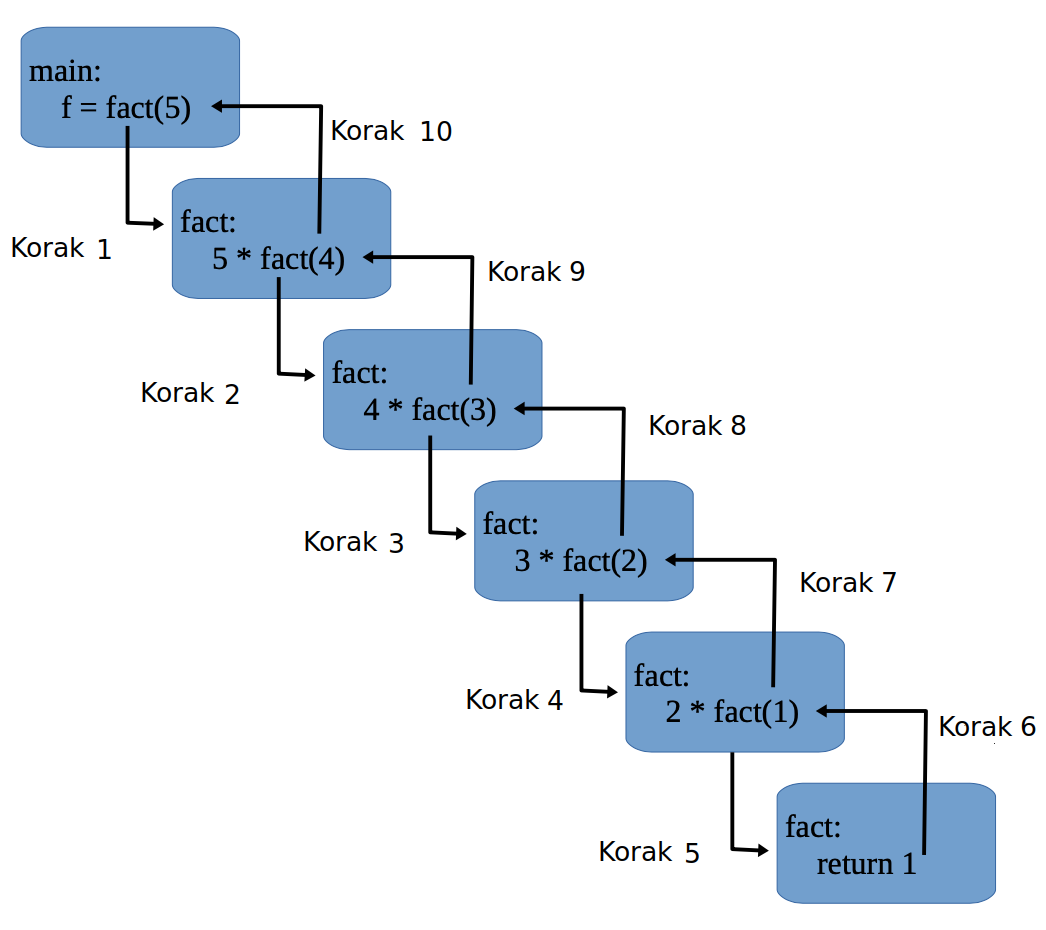
\includegraphics[width=220pt,height=140pt]{slike/factorial_recursion_tree.png} 
	\label{fig:rec_tree}
	\caption{Drvo rekurzije.}
\end{figure}

 


\textit{Kompleksnost rekurzije}. Jasno je da je kompleksnost ove rekurzije linearna, tj. $O(n)$. \\ \vspace{0.2cm}


Ako bazni slučaj nije dostignut ili nije definisan, može doći do problema  prekoračenja steka (eng. \textit{stack overflow}). Posmatrajmo sljedeći program.

\begin{minted}{python}
	def fact(n):
	# pogrešan bazni slučaj 
	if (n == 100): 
	    return 1	
	else:
	    return n*fact(n-1);
\end{minted}

Ovaj program će izazvati prekoračenje steka u slučaju kada je ulaz $n<100$;  tada bazni slučan nikada neće biti ispunjen i rekurzija će se pozivati dok god se ne iscrpi memorija steka rezervisana za program.

\section{Vrste rekurzija}

Funkciju  nazivamo \textit{direktnom} rekurzivnom ako ona poziva istu funkciju. Funkcija \texttt{fun} se naziva \textit{indirektnom} rekurzivna ako poziva drugu funkciju koja potom poziva direktno ili indirektno funkciju \texttt{fun}. Razlika između direktne i indirektne rekurzije ilustrovana je data u narednom programu.

\begin{minted}{python}
	# Direktna rekurzija
	def direktnaRecFunc():
	    # Kod ....
	
	    direktnaRecFunc()
	
	    # Kod...
	
	# Indirektna rekurzija
	def indirektnaRecFun1():
	    # Kod ...
	
	    indirektnaRecFun2()
	
	    # Kod...
	
	def indirektnaRecFun2():
	
	    # Kod...
	
	     indirektnaRecFun1()
	
	     # Kod...
\end{minted}



Rekurzivna funkcija se naziva \textit{repnom} rekurzijom ako je rekurzivni poziv posljednji dio koda koju funkcija izvršava. Inače, rekurzivna funkcija se naziva \textit{nerepnom}.
 
\subsection{Prednosti i nedostaci rekurzivnog nad iterativnim pristupom}

Svaka rekurzija se može napisati na ekvivalentan, iterativni pristup. 
Iako rekurzija i iteracija u ugnježdenim petljama na prvi pogled djeluju dosta slično postoje značajne, suštinske razlike:
\begin{itemize}
	\item Rekurzija se prekida kada se dostigne bazni slučaj; iteracija se prekida kada uslov postane netačan.
	\item Rekurzija se veže za funkcije, dok se iteracija veže za petlje.
	\item Svaki rekurzivni poziv zahtijeva dodatni prostor koji se alocira u memoriji steka; iteracija ne zahtjeva dodatni memorijski prostor.
	\item Rekurzija najčešće ima kraći k\^od; iteracije u petlji su često obimnijeg k\^oda. 
	
\end{itemize}


%Iz ranijih kurseva osnova programiranja je poznato da rekurzivni i iterativni programi imaju istu moć rješavanja problema, tj. svaki rekurzivni program može se napisati u  iterativnom obliku i obrnuto. 

Rekurzivni program ima veće zahtjeve za prostorom od (ekvivalentnog) iterativnog programa, jer će sve funkcije ostati na steku dok se ne dostigne bazni slučaj. Takođe,  zahtjevi za vremenom su veći zbog poziva funkcija i   troškova vraćanja rezultata. Dodatno, zbog manje dužine k\^oda, kodovi znaju biti teški za razumevanje i stoga je potrebno uložiti  dodatnu pažnju prilikom pisanja k\^oda zbog mogućih previda. %Računar može ostati bez memorije ako rekurzivni pozivi nisu ispravno provjereni.

Prednost korištenja rekurzija je u čistom i jednostavnijem načinu pisanja k\^oda. Neki problemi su inherentno rekurzivni, npr. obilazak stabala, problem hanojskih kula, itd. Za takve probleme, poželjno je, a i intuitivnije,  pisati rekurzivni k\^od. Kako smo već naveli, takve kodove možemo pisati i iterativno uz pomoć strukture podataka steka.

\subsection{Primjene rekurzivnog pristupa}

Rekurzija je moćna tehnika sa raznim primjenama u informatici i programiranju. Neke od uobičajenih primjena rekurzije uključuju:

\begin{itemize}
	\item  \textit{Prelazak stabla i grafa}. Rekurzija se često primjenjuje za prelazak i pretraživanje značajnih struktura podataka kao što su stabla i grafovi. Rekurzivni algoritmi se mogu koristiti za istraživanje svih čvorova ili vrhova stabla ili grafa na sistematičan način.
	\item \textit{Algoritmi za sortiranje}. Rekurzivni algoritmi se koriste u algoritmima za sortiranje kao što su \textit{quick sort} (brzo sortiranje) i  \textit{merge sort} (sortiranje spajanjem). Ovi algoritmi koriste rekurziju da podijele podatke u manje podliste, sortiraju ih, a zatim ponovo spajaju.
	%\item \textit{Algoritmi zavadi pa  vladaj}: Mnogi algoritmi koji koriste pristup zavadi pa vladaj, kao što je algoritam binarnog pretraživanja, koriste rekurziju da razbiju problem na manje podprobleme.
	\item \textit{Generisanje fraktala}.  Fraktalni oblici i obrasci mogu se generirati korištenjem rekurzivnih algoritama. Npr. Mandelbrotov skup se generiše uzastopnom primjenom rekurzivne formule na kompleksne brojeve.
	
	\begin{figure}
		\centering
		
\includegraphics[width=100pt,height=80pt]{slike/mandelbrot.png}
		\caption{ Mandelbrotov skup}
	\end{figure}


	\item \textit{Algoritmi vraćanja unazad}. Algoritmi vraćanja unazad se koriste za rješavanje problema koji uključuju donošenje niza odluka, gdje svaka odluka zavisi od prethodnih. Ovi algoritmi se mogu implementirati korištenjem rekurzije za istraživanje svih mogućih staza i vraćanje unatrag kada se rješenje ne pronađe.
	\item \textit{Memoizacija}.  Ovo je tehnika koja uključuje pohranjivanje rezultata skupih poziva funkcija i vraćanje keširanih rezultata kada se naiđe na pozive funkcija istih ulaza. Memoizacija se može implementirati korištenjem rekurzivnih funkcija koje izračunavaju i keširaju rješenja podproblema.
\end{itemize}

\subsection{Primjena rekurzivnog pristupa  }

Pogledajmo naredni zadatak (o rastu populacije zečeva kroz vrijeme). 
\begin{example}
  
	Pretpostavimo da se zečevi reprodukuju na sljedeći način: par zečeva se na kraju prvog mjeseca života ne razmnožava. Međutim, na kraju drugog i svakog sljedećeg mjeseca oni reprodukuju novi par zečeva. Postavlja se pitanje koliko će novorođenih parova zečeva biti poslije godinu dana (tj. na kraju 12-og mjeseca)?
\end{example}

\begin{solution}
	 
	
	Brojevi parova zečeva čine niz: $0, 1,1, 2,3,5,8,13, 21, \ldots$ 
	
	Lako zaključavamo da je svaki sljedeći broj u nizu jednak zbiru prethodna dva broja, tj. ako je $f(n)$ broj  novorođenih zečeva na kraju $n$-tog mjeseca, onda je 
	$$f(n) = f(n-1) + f(n-2), n \geq 2$$
	gdje je bazni slučaj dat sa $f(0)= 0, f(1) = 1$.
\end{solution}

Ova rekurzija je implementirana sljedećim (Pajton) kodom.

\begin{minted}{python}
	def fib(n):
		if n == 0:
			return 0
		if n == 1:
			return 1
		return fib(n-1) + fib(n-2)
\end{minted}

Dakle, u svakom koraku, ako se ne dođe do trivijalnog koraka, rekurzivni poziv će pozvati dvije nove rekurzije (sa manjim veličinama ulaza). Potom će, vraćanjem rezultata na manjim ulazima, rezultat biti izračunat i za veće ulaze. Rješenje prethodnog zadatka se dobija račinajuću rekurziju za ulaz $n=12$. 

%https://www.quora.com/What-is-the-time-complexity-of-the-simplest-recursive-algorithm-that-finds-the-nth-Fibonacci-number
\textit{Kompleksnost algoritma}. Primijetimo da se u svakom koraku broj poziva duplira u odnosu na prethodni. Brzina opadanja veličine ulaza opada konstantno u odnosu na $n$, pa zaključujemo da je kompleksnost izvršavanja rekurzije eksponencijalna, tj. jednaka $O(2^n)$.

%fib_rec.jpeg
\begin{figure}[H]
	\centering
	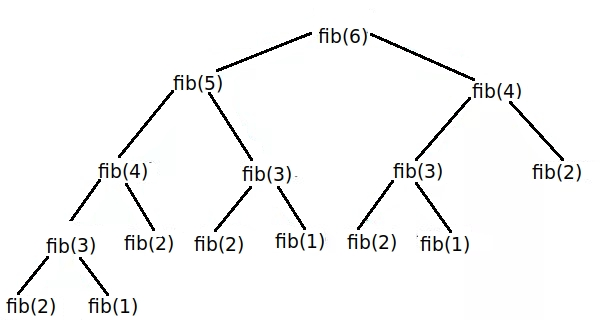
\includegraphics[width=250pt,height=140pt]{slike/fib_rec.jpeg} 
	\label{fig:rec_fib}
	\caption{Drvo rekurzije za \texttt{fib} rekurzivni metod.}
\end{figure}



 %https://www.geeksforgeeks.org/c-program-for-tower-of-hanoi/
 \begin{example}
 	\textbf{\emph{Problem Hanojskih kula}}. Neka su data tri štapa i $n$ diskova. Zadatak ovog problema je u što manje poteza
 	premjestiti diskove sa jednog štapa na drugi štap. Sljedeća pravila vrijede pri prebacivanju diskova. 
 	\begin{itemize}
 		\item Inicijalno, diskovi stoje poredani na jednom štapu ($A$) jedan na drugi gdje  manji diskovi stoje na većim diskovima (pretpostavka je da su diskovi različitih dimenzija). 
 		\item Potez se sastoji od premiještanja jednog diska sa vrha jednog štapa na vrh drugog štapa.   
 		\item Veći disk ne može nikada da bude stavljen na manji disk u bilo kojoj iteraciji premiještanja.
 	\end{itemize}
  \end{example}    

\begin{solution}
 
 
 	Situacija sa dva diska i tri štapa je jasna. Pretpostavimo da se dva diska inicijalno nalaze na štapu $A$ i da ih želimo premijestiti na štap $C$, poštujući uslove zadatka. Označimo ta dva diska crvenom (veći disk) i plavom (manji disk). U prvomu korak prebacujemo plavi disk na štap $B$. Potom crveni disk prebacujemo na štap $C$. Konačno, plavi disk sa štapa $B$ prebacujemo na štap $C$, čime je zadatak završen za slučaj sa dva diska ($n=2$).
 	
 	Posmatrajmo situaciju sa kulama kao na Slici~\ref{fig:tower} sa tri diska ($n=3$) i tri štapa ($A, B$ i $C$). 
 	
 	\begin{figure}[H]
 		\centering
 		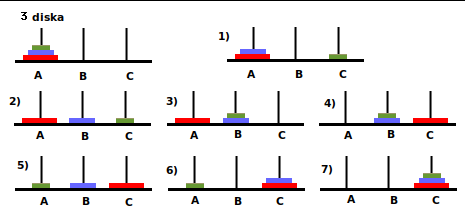
\includegraphics[width=270pt,height=150pt]{slike/tower.png}


 	 \caption{Problem hanojskih kula, $n=3$ diska.}     \label{fig:tower}
 	 	\end{figure}

 Prvo se najmanji (zeleni) disk prebacuje na štap $C$. Drugi korak je prebacivanje plavog (disk srednje veličine) na štap $B$. Potom, u koraku tri, zeleni disk sa štapa $C$ premiještamo na štap $B$. Korak četiri je rezervisan za prebacivanje najvećeg diska (sa štapa $A$)  na štap $C$. Dalje, potom zeleni disk sa $B$ premiještamo na štap $A$, a plavi na štap $C$. Konačno, u koraku sedam, zeleni disk sa štapa $A$ prebacujemo na štap $C$.  
 
Označimo sa $T(n)$ broj koraka koji je potreban da prebacimo $n$ diskova sa štapa $A$ na štap $C$ koriteći pomoćni štap $B$. Bazni slučaj je $T(1) = 1$. Izvedimo rekurzivni korak za ovaj problem. Kako smo pomenuli, ideja rekurzije je svesti početni problem na rješavanje problema manjih dimenzija (podprobleme) koje ponovo   rekurzivno rješavamo. U ovom slučaju, ``hvatamo'' se za činjenicu da ukoliko je najveći disk sam na jednom štapu, ostalih $n-1$ diskova sa drugog štapa možemo nesmetano prebacivati koristeći sva tri štapa (na veliki disk može da se stavi bilo koji od $n-1$ diskova). Rekurzivno prebacimo $n-1$ diskova sa vrha štapa $A$ na štap $B$, koristeći štap $C$. Nakon toga, situacija je  sljedeća: ($i$) najveći disk se nalazu na štapu $A$; ($ii$) ostalih $n-1$ diskova su složeni na štapu $B$; ($iii$) štap $C$ je prazan. Sljedeći korak je prebacivanje najvećeg diska sa štapa $A$ na štap $C$. Nakon toga, ponovo rekurzivno prebacujemo $n-1$ diskova sa štapa $B$ na štap $C$, koristeći štap $A$. Prema tome, vrijedi rekurzija:
$$ T(n) = 2 \cdot T(n-1) + 1, T(1) = 1.$$
 
Implementacija rekurzivnog pristupa problema Hanojskih kula je data sljedećim k\^odom. 

\begin{minted}{python}
	 
	def TowerOfHanoi(n , izvor, cilj, pomocni):
	    if n==1:
	        print ("Pomaknite disk 1 sa štapa ", izvor," \ 
	        na štap ", cilj)
	        return
	    TowerOfHanoi(n-1, izvor, pomocni, cilj)
	    print ("Pomakni disk ",n," sa štapa ", izvor," na štap  \ 
	     ", cilj) #pomijeranje najvećeg štapa
	    TowerOfHanoi(n-1, pomocni, cilj, izvor)
	
	#instanca:
	n = 4 #broj diskova
	TowerOfHanoi(n, 'A','B','C')
\end{minted} 

\textit{Vremenska kompleksnost}. Vrlo lako dobijamo eksplicitnu funkciju koja odgovara   rekurzivnoj relaciji problema: $T(n)= 2  T(n-1) + 1 = 2 \cdot ( 2 \cdot T(n-2) + 1) + 1 = \cdots = 2^{n-2} + 2^{n-1} + \cdots + 2 + 1 = 2^n -1.$
Rekurzija se izvrašava u $O(2^n)$ vremenu.  %Prema tome, $T(n) = O(2^n)$, što je eksponencijalno vrijeme izvođenja. 


\end{solution}	
 

\section{Algoritmi grube sile}
%Literatura: https://www.geeksforgeeks.org/most-important-type-of-algorithms/
%https://stanford-cs161.github.io/winter2023/assets/files/lecture2-notes.pdf

%https://www.khanacademy.org/computing/computer-science/algorithms/asymptotic-notation/a/big-o-notation ==> Zadaci

% https://textbooks.cs.ksu.edu/cc310/4-data-structures-and-algorithms/12-brute-force/

Jedna od prvih algoritamska tehnika koja se koristiti u rješavanju  računarskih problema je tehnika grube sile. Ovo je algoritamska paradigma sa kojom se većina čitalaca susretala do sada, mada možda nesvjesno da je riječ o baš toj tehnici rješavanja problema.

Prosto rečeno, paradigma grube sile pokušava sva moguća rješenja problema, vraćajući ono koje je najbolje (ili prvo koje zadovoljava uslove zadatka, ako je riječ o problemima zadoovljenja -- tzv. SAT problemi). U stvarnom životu,  primjer algoritma brutalne sile je uključivanje USB kabela. Prvo pokušamo  na jedan način, a ako to ne uspije, isprobamo drugi port.  Slično, ako imamo veliki broj ključeva, a nismo sigurni koji od njih otključava vrata, možemo jednostavno isprobati svaki ključ za datu bravu dok jedan ne proradi. Upravo je ovo suština algoritamskog dizajna ove paradigme.

\begin{example}
	Odličan primjer algoritma grube sile je pronalaženje najbližeg para tačaka u višedimenzionalnom (realnom) prostoru. Neka su date $n$ tačaka u $\mathbb{R}^m$, tj. $S=\{ \textbf{x}_i \mid \textbf{x}_i \in  \mathbb{R}^m, i=1, \ldots, n\}$. Naći dvije tačke $x_i, x_j \in S$ koje su međusobno najbliže gledajući sve parove tačaka skupa $S$.
\end{example}
\begin{solution}
    Da bismo pronašli odgovor grubom silom,  izračunamo udaljenost između svakog pojedinačnog para tačaka, a zatim pratimo minimalnu pronađenu udaljenost. Verzija ovog algoritma je data narednim k\^odom.
   
\footnotesize{
\begin{minted}{python}
	import math 
	def min_dist_par(S):
		min_dist = float('-inf')
		point1 = None	
		point2 = None
		for p1 in S:
			for p2 in S:
				if p1 != p2:
					distance = math.dist(p1, p2)
					if distance < min_dist:
					     min_dist = distance
    			 		point1 = p1
    			 		point2 = p2
\end{minted}}
\end{solution}

\textit{Kompleksnost algoritma}. Kako je $|S| = n$, lako se primijeti da je broj parova tačaka jednak $O(n^2)$. Dalje, računanje (euklidove) udaljenosti između dvije $m$-dimenzionalne tačke se izvršava u $O(m)$ vremenu. Prema tome, ukupno vrijeme izvršavanja je $O(n^2)\cdot O(m) = O(n^2\cdot m) = O(n^2)$, jer je $m$ konstantno.

\begin{example}
	Riješimo problem ruksaka uz pomoć algoritma brutalne sile. Ovaj problem je definisan na sljedeći način: Neka je dato $n$ proizvoda i svaki do njih ima svoju težinu $w_i$ i cijenu (vrijednost) $p_i, i=1,\ldots, n$. Ruksak ima kapacitet $C>0$. Koji od proizvoda staviti u ruksak, tako da cijena bude najveća, ali da   kapacitet ruksaka ne bude narušen. 
\end{example}

\begin{solution}
	Posmatrajmo primjer instance problema.
\begin{center}	
	\begin{tabular}{ccc}
		\emph{proizvod} & \emph{težina} & \emph{cijena} \\ \hline
		1        &  2	& 20 \\
		2		& 	5	& 30 \\
		3		& 10	& 50 \\
		4		&  5 	& 10 \\ \hline
	\end{tabular}
\end{center}
Neka je kapacitet ruksaka $C=16$.


\end{solution}

Enumeracijom prostora mogućih rješenja (kojih ima ukupno $2^4=16$), dobijamo sljedeću tabelu.
\begin{center}
	\begin{tabular}{lcl}
     Rješenja (proizvodi u ruksaku) & Ukupna težina & Ukupna cijena \\ \hline
	$\{1\}$	&   2     &  20 \\
	$\{2\}$ &	5	  &  30 \\
	$\{3\}$ &	10    &  50 \\
 	$\{4\}$ &    5	  &  10 \\
	$\{1,2\}$ &	 7    &  50 \\
	$\{1,3\}$  &  12  &  70 \\
    $\{1,4\}$  &   7  &  30 \\
    $\{2,3\}$  & 15   &  80 \\
    $\{2,4\}$  & 10   &  40 \\
     $\{3,4\}$ & 15   &  60 \\
     $\{1,2,3\}$  &17  & nedopustivo \\
     $\{1,2,4\}$  & 12 & 60 \\
      $\{1,3,4\}$ & 17 & nedopustivo \\
      $\{2,3,4\}$ & 20 & nedopustivo \\
      $\{1,2,3,4\}$ & 22 &  nedopustivo \\ \hline
	\end{tabular}
\end{center}
Iz prethodne tabele, lako se vidi da je najbolje odabrati proizvod 2 i 3 i staviti ih u ruksak. Pri tome, njihova   cijena je 80. Primijetimo da  rješenje koje uzima proizvode 1, 2 i 3 u ruksak narušava njegov kapacitet (težina je 17, što je veće od 16). 

Jasno je da je skup rješenja problema ruksaka poistovijećen sa pretraživanjem svih podskupova skupa $[n]$.  Prema tome, kompleksnost ovakvig pristupa je eksponencijalna, tj. $O(2^n)$. Pristup je dat sljedećim 
kodom. 

%\footnotesize
\begin{minted}{python}
	  best_fitness: float = 0.0
	  
	  #instance example:
	  N = 4
	  w = [2, 5, 10, 5]
	  p = [20, 30, 50, 10]
	  C = 16
	  # helper function
	  def objective(solution):
	  
	  	if len(solution) == 0: 
	  		return float('-inf')
	  	fitness: float = 0.0
	  	weight: float = 0.0
	  
	  	for i in solution: 
	  		fitness += p[i]
	  		weight += w[i]
	  
	  	if weight > C:
	  		return float('-inf')
	  	else:
	  		return fitness
	  
	  # brute force recursion
	  def knapsack_brute_force(solution): 
	  	global best_fitness
	  
	  	if objective(solution) > best_fitness:
	  		best_fitness = objective(solution) 
	  
	  	for i in range(N):
	  		if  len(solution) >= 1: 
	  			if i > max(solution) : # symmetry breaking 
	  				#print(solution + [i])
	  				knapsack_brute_force(solution + [i]) 
	  		else:
	  			knapsack_brute_force(solution + [i]) 
	  
	  knapsack_brute_force([])
	  print(best_fitness) # 80.0	
	  
\end{minted}


Kako primjećujemo na osnovu prethodne (rekurzivne) implementacije, svaki od  
rekurzivnih poziva, kojih je tačno $2^n$, poziva funkciju \textit{objective}. Preciznije, kompleksnost pristupa brutalne sile je $O(2^n)$. Napomenimo da postoje dosta efikasniji pristupi za rješavanje problema ruksaka. Među njima, izdvajamo metod dinamičkog programiranja, o kojem će biti više riječi u nastavku.


\section{Algoritmi pretraživanja}
% https://www.geeksforgeeks.org/searching-algorithms/
\textit{Algoritmi pretraživanja} su dizajnirani sa zadatkom provjeravanja da li se element nalazi (ili da se vrati) u strukturi podataka u kojoj je on pohranjen; takođe,  da se vrati poruka ako takav element ne postoji.

Ovi algoritmi se generalno dijele u dvije kategorije na osnovu načina pretraživanja:

\begin{itemize}
	\item \textit{Sekvencijalna pretraga}: U ovom slučaju se lista ili niz prelazi uzastopno i svaki element se provjerava; primjer ovakve pretrage je \textit{linearna pretraga}.
	\item \textit{Intervalna pretraga}: Ovi algoritmi su   dizajnirani za pretraživanje u sortiranim strukturama podataka; mnogo su efikasniji od linearne pretrage jer dijele prostor pretraživanja na dijelove,  pokušavajući na taj način eliminisati veliki dio prostora za pretragu svakom iteracijom. Primjer takve pretrage je \textit{binarna pretraga}.
\end{itemize}

\subsection{Linearna pretraga}
Ovo je sekvencijalna pretraga, koja pretražuje (nizovne) strukture tako što prolazi kroz svaki njeni element dok se ne pronađe željeni element,  ili se ne dođe do kraja skupa podataka strukture (tj. svi elementi strukture su posjećeni pretragom).  Iterativna implementacija linearne pretage je data sljedećim k\^odom.

\begin{minted}{python}
	def search(arr, x):
	
	  for i in range(len(arr)):
	      if (arr[i] == x):
	          return i
	  return -1
	
	arr = [2, 3, 1, 11, 10, 20]
	x = 10
	
	res  = search(arr,  x)
	if(result == -1):
	    print("Element nije prisutan")
	else:
	    print("Element je prisutan pod indeksom ", res)
\end{minted}
%https://www.geeksforgeeks.org/linear-search/: LINEARNA PRETRAGA
\textit{Kompleksnost algoritma}. Lako se vidi da je kompleksnost linearne pretrage upravo linearna, $O(n)$, gdje je $n$ veličina (nizovne) strukture. 

Implementacija rekurzivnog pristupa za linearnu pretragu je data narednim k\^odom.

\begin{minted}{python}
	def linear_search(arr, x, n):
	if n >= len(arr):
	    return -1
	
	if arr[n] == x:
	   return n
	
	return linear_search(arr, x, n+1)
	
	#poziv 
	res = linear_search(arr,x,0)
	
\end{minted}

Vremenska složenost je $O(n)$ dok se za rekurzivni pristup izdvaja i pomoćni prostor kompleksnosti $O(n)$, za alokaciju prostora steka tokom izvođenja rekurzivnih poziva.


Linearna pretraga nije efikasna za nizove velikih dimenzija i koristi se samo kada radimo sa malim skupom podataka, te kada želimo da algoritam držimo što jednostavnijim.
\subsection{Binarna pretraga}
% https://www.geeksforgeeks.org/binary-search/: BINARNA PRETRAGA

Za upotrebu binarnog pretraživanja u bilo kojoj strukturi podataka, struktura podataka mora imati sljedeća svojstva: ($i$) treba biti sortirana; 
($ii$) pristup bilo kojem elementu strukture podataka se odvija u konstantnom vremenu.

Ideja binarne pretrage se sastoji u eksploatisanju svojstva da je niz sortiran. Pretpostavimo bez smanjenja opštosti da je niz sortiran u rastućem poretku. To znači da u slučaju da se na indeksu $i$ nalazi element veći od traženog elementa $x$, $x$ se (potencijalno) nalazi lijevo od indeksa $i$, te indekse $i+1, \ldots$ isključujemo dalje iz razmatranja. U svakoj iteraciji, biramo indeks $i$ kao središnji element niza, koji se potom poredi sa $x$. U zavisnosti od rezultata, imamo tri mogućnosti: ($i$) element na poziciji $i$ je upravo $x$, čime prekidamo pretragu vraćajući dati indeks; ($ii$)  element na poziciji $i$ je veći od $x$, čime pretragu usmjeravamo na elemente niza lijevo od pozicije $i$; ($iii$) inače, pretraga se seli na desni dio niza, tj. elemente čiji je indeks veći od $i$. Za bazne slučajeve uzimamo kada je niz veličine 0 ili 1. U provom slučaju vraćamo \textit{False}, dok u drugom slučaju vraćamo rezultat poređenja elementa niza sa $x$.  

Implementacija rekurzivnog pristupa binarne pretrage je data sljedećim k\^odom.

\begin{minted}{python}
	def binary_search(arr, x):
	   
	    if len(arr) == 0:
	       return False
	        
	    if len(arr) == 1:
	       return True if arr[0] == x else False

	    mid = len(arr) // 2
	    if arr[mid] == x:
	       return True
	    elif arr[mid] < x:
	         return binary_search(arr[mid+1:], x)
	    else: 
	         return binary_search(arr[:mid], x)

    # pozivanje programa:
    arr = [2, 8, 10, 12, 15]
    x = 2
    pos = binary_search(arr, x)
    print(pos)
\end{minted} 

\textit{Kompleksnost algoritma}. Broj interacija u rekurziji koju zadovoljava binarna pretraga je $T(n) = T(n/2) + c$, gdje je $c=O(1)$. na osnovu Master teoreme, kompleksnost algoritma je jednaka $O(\log n)$. 

Binarnu pretragu koristimo u situacijama kada pretražujemo veliki skupa  podataka, jer ima vremensku složenost od $O(\log n)$, dakle, mnogo brže od linearne pretrage. Pri tom  skup podataka treba biti sortiran.
Bitno je i da podaci u nizu nemaju složenu strukturu ili odnose između sebe, jer to narušava efikasnost pretrage te kompleksnost rješavanja ne mora više ne bude logaritamska.  

%https://www.geeksforgeeks.org/jump-search/: JUMP SEARCH
\subsection{Pretraga preskakanjem}

Kod ove pretrage se takođe podrazumijeva da je niz sortiran.  Osnovna ideja je sistematskom provjerom razumnog broja elemenata niza,  koristeći preskakanje nekih elemenata umjesto pretraživanja svih elementa  ustanoviti uži interval u kojem se dati element $x$ traži.

Pretpostavimo da imamo niz \emph{niz} veličine $n$ i dužinu bloka (elemenata) veličine $m$ koji koristimo kao korak preskakanja. Pretraga prvo pretražuje elemente $niz[0], niz[m]$, $niz[2m] \ldots niz[k \cdot m]$ i tako dalje. Kada pronađemo interval (indekse) sa svojstvom $niz[k\cdot m] < x < niz[(k+1) \cdot m]$, izvodimo operaciju linearne pretrage elementa $x$ na intervalu dužine $m$.  %, krenuvši sa indeksom $k\cdot m$ u svrhu  pronaska elementa $x$.
 
 
 Razmotrimo sljedeći \emph{niz}$=[0, 1, 1, 2, 3, 5, 8, 12, 24, 37, 55, 82, 140, 433, 567, 622]$. Preskakanjem pronalazimo vrijednost $x=55$, za veličinu koraka preskakanja $m=4$. Sljedeće iteracije se izršavaju. 
 \begin{itemize}
 	\item  Skok sa indeksa 0 na indeks 4;
 	\item   Skok sa indeksa 4 na indeks 8;
 	\item   Skok sa indeksa 8 na indeks 12;
 	\item  Pošto je element na indeksu 12 veći od 55, skočit ćemo korak unazad da bismo došli do indeksa 8;
 	\item  Izvršite linearnu pretragu iz indeksa 8 da bismo našli element 55.
 \end{itemize}
 
 \textit{Kompleksnost algoritma}. U najgorem slučaju, moramo uraditi $n/m$ skokova, a ako je posljednja provjerena vrijednost veća od elementa koji se traži, vršimo $m-1$ poređenja više za linearnu pretragu. Stoga je ukupan broj poređenja u najgorem slučaju jednak $((n/m) + m-1)$. Vrijednost ove funkcije  je minimalna kada je $m = \sqrt{n}$, što i predstavlja najbolju vrijednost za peskakanje. Dakle, u najboljem slučaju, kompleksnost algoritma je $O(\sqrt{n})$. 
 
 
Relurzivna implementacija pretage preskakanjem  je data sljedećim kodom   u jeziku Pajton. 
 
 \begin{minted}{python}
 def jump_search(niz, x, jump, k):
 
 	if k * jump >= len(niz): #empty array
 		return False
 
 	if k * jump < len(niz) and (k+1) * jump >= len(niz): 
 		found = linear_search(niz[k*jump :], x, 0)
 		return found
 	#rekurzivni korak: oba kraja intervala su elementi niza: 
 	if niz[ k * jump ] <= x and x <= niz[ (k+1) * jump ]:
 		found = linear_search(niz[k*jump: ((k+1)*jump + 1)], x, 0)
 		return found
 	else:
 		return jump_search(niz, x, jump, k+1) # idemo na naredni interval
 
 	#instanca:
 	niz = [2, 10, 21, 33, 38, 41, 45, 52, 57, 70, 75]
 	jump_step = 3
 	x= 57
 	# poziv metoda:
 	found = jump_search(niz, 57, jump_step, 0)
 	print(found) 
 \end{minted}

\subsection{Interpolacijska pretraga}

% https://www.geeksforgeeks.org/interpolation-search/  

 Interpolacijska pretraga je poboljšanje  binarnog pretraživanja   gdje pretpostavljamo da su vrijednosti u sortiranom nizu uniformno (ravnomjerno) raspoređene. Interpolacija konstruiše nove tačke   unutar opsega diskretnog skupa strukutre podataka. Kao što znamo, binarno pretraživanje uvijek polazi sa provjerom srednjeg elementa niza. Sa druge strane, interpolacijska pretraga može tražiti na različitim mjestima u strukturi. Npr. ako je vrijednost traženog elementa  bliža posljednjem elementu, interpolacijska pretraga će vjerovatno započeti pretragu više prema krajnjoj strani strukture.
  
  Za pronalazak pozicije  \emph{pos} u nizu \emph{niz}, koristi se sljedeća ideja: vraćamo višu vrijednost \emph{pos} ako je element koji se traži bliži kraju niza, tj. $niz[n-1]$. Manja vrijednost za \emph{pos} se vraća kada je vrijednost bliže početku niza, tj. elementu $niz[0]$. 
  
  Poziciju \emph{pos} računamo po sljedećoj formuli:
  \begin{equation}\label{eq_interpolation-search-formula}
     pos = \left \lfloor \frac{ (n-1)}{ niz[n-1] - niz[0]}\cdot(x - niz[0]) \right \rfloor
  \end{equation}
  Algoritam se sastoji od sljedećih koraka:
  \begin{enumerate}
  	\item  Izračunamo vrijednost \emph{pos} koristeći formulu (\ref{eq_interpolation-search-formula}).
  	\item Ako se vrijednost podudara sa traženom, vraćamo indeks/vrijednost \textit{True} i izlazimo iz rekurzije.
  	\item Ako je traženi element manji od $niz[pos]$, interpoliramo poziciju \emph{pos} lijevog podniza. U suprotnom, interpoliramo poziciju \emph{pos} desnog podniza.
  	\item Ponavljati korake 1-3, sve dok se ne pronađe podudaranje ili dok podniz ne postane prazan.
  \end{enumerate}

Implementacija reekurzivnog pristupa interpolacijske pretrage je data narednim k\^odom. 
\begin{minted}{python}
	def interpolation_search(niz, l, r, x):

		if (lo <= hi and x >= niz[l] and x <= niz[r]):
			pos = l + ((r - l) // (niz[r] - niz[lo]) * \ 
			(x - niz[l]))
	
			if niz[pos] == x:
				return pos
	
			#desni podniz
			if niz[pos] < x:
				return interpolation_search(niz, pos + 1, r, x)
	
			#lijevi podniz
			if niz[pos] > x:
				return interpolation_search(niz, l, pos - 1, x)
		return -1
\end{minted}

\textit{Kompleksnost algoritma}. Algoritam u najgorem slučaju postiže vrijeme od $O(n)$.  Može se pokazati da je očekivano vrijeme izvršavanja ovog algoritma mnogo bolje, i iznosi $O(\log \log n)$.

\subsection{Eksponencijalna pretraga}

Naziv ovog algoritma potiče iz načina biranja sljedećeg elementa u pretrazi. 


Eksponencijalna pretraga uključuje dva koraka. Prvo, pronađimo interval u kojem se element potencijalno nalazi (ako se nalazi) koristeći eksponencijalne korake. Potom, na datom intervalu primijenimo binarnu pretragu. Za  poziciju \emph{pos} uzimamo $0, 2, 4, \ldots$ dok ne nađemo indeks  $i$ tako da je traženi element $x$ veći ili jednak od elementa  na poziciji $2^{i-1}$ a manji ili jednak od elementa na poziciji $2^i$ niza koji se pretražuje. 


   Implementacija ove pretrage je data narednim kodom koji je napisan u jeziku pajton. 
   
   \begin{minted}{python}
   def exponential_search(niz, x, l):
   
   	if len(niz) <= 1:
   	  if x in niz:
   		 return  l + int(x in niz)
   	  else:
  		 return -1 
   
   	  if l == 0:
   		 pos = 2
   	  else:
   		 pos = l * 2
   
   	  if pos >= len(niz):
   		 ind_found = binary_search(niz[l:], x)
		 # ako x ne postoji u sufiksu
   		 if ind_found == -1:  
   			return -1
   		 else:
   			 return l + binary_search(niz[l:], x)
   	  else:
   		 if niz[l] <= x and x <= niz[pos] :
   		    return l + binary_search(niz[l: pos+1], x)
   		 else:
   		    return exponential_search(niz, x, pos)
   # instanca:
   niz = [2, 10, 22, 38, 44, 51, 100, 220, 550, 880]
   x = 10
   # poziv funkcije: 
   print(exponential_search(niz, x, 0))
   \end{minted}

\textit{Kompleksnost algoritma}.  Ovaj algoritam pripada klasi $O(\log n)$. 
 

Eksponencijalna pretraga je posebno korisna za pretraživanja u kojima je  veličina niza ogromna.  Ova pretraga se pokazala efikasnijom   od binarnog pretraživanja za ograničene nizove (maksimalni element je unaprijed ograničen nekom konstantom), a takođe i kada je element koji se traži bliži prvom elementu.

\section{Algoritamska paradigma podijeli pa zavladaj}
%https://textbooks.cs.ksu.edu/cc310/4-data-structures-and-algorithms/13-divide-and-conquer/
Ideja ovog (rekurzivnog) prostupa je sljedeća:
\begin{itemize}
	\item  Podijelimo problem   na nezavisne podprobleme efikasno;
	\item Riješimo podprobleme rekurzivno;
	\item  Kombinujmo rješenja podproblema na efikasan način, tako da rezultat ostane validan i za veći podproblem.
\end{itemize}

Pseudokod date paradigme je dat  Algoritmom~\ref{alg:d-n-c}. 

%https://cgi.csc.liv.ac.uk/~ped/teachadmin/algor/algor_complete.html
  

\begin{algorithm}
	
\begin{algorithmic}[1]
\Procedure{D\&C}{$n$: veličina ulaza}
 
  \If{ $n < = n_0$}
  \State Riješiti problem bez dodatnog dijeljenja 
  \Else
 
   \State Podijeliti problem na $r$ podproblema svaki veličine $\approx n/k$;
    \For{svaki od $r$ podproblema}
        \State Pozovemo D\&C ($n/k$)
     \EndFor
   \State Kombinujmo $r$ rezultujućih rješenja podproblema da bi se dobilo rješenje početnog problema
\EndIf
\EndProcedure
\end{algorithmic}

\caption{Pseudokod algoritamske paradigme Zavadi pa vladaj.}\label{alg:d-n-c}
\end{algorithm}
Dobro poznati primjer gdje se ova algoritamska paradigma primjenjuje je sortiranje spajanjem, gdje se sortiranje $n$ brojeva odvija u $n \log n$ vremenu. 

Ideja sortiranja niza je sljedeća:
\begin{itemize}
	\item  Podijeliti niz na dva (podjednaka), disjunktna, dijela -- lijevi i desni;
    \item Sortirati rekurzivno oba dijela niza;
    \item Spojiti dva sortirana niza u linearnom vremenu.
\end{itemize}

Izvorni kod za sortiranje spajanjem u programskom jeziku Pajton je dat u nastavku.
\begin{minted}{python}
 def mergeSort(niz):  

   if len(niz) <= 1:    
	 	return niz
   else:
      ##partition:
      nizLeftSort = niz[0 : (len(niz)//2) ]
	  nizRightSort = niz[ (len(niz) // 2) :] 
	  mergeSort(nizLeftSort) 
	  mergeSort(nizRightSort)
	  ## combine
	  niz.clear()
	  indexL = indexR =  0
	  while(indexL < len(nizLeftSort) and indexR < len(nizRightSort)):
	 	 if(nizLeftSort[ indexL ] >= nizRightSort[ indexR ]):
	 		 niz.append(nizLeftSort[indexL])
	 		 indexL = indexL + 1
	 	 else:
	 		 niz.append(nizRightSort[indexR])
	 		 indexR = indexR + 1
	 
	  if(indexL < len(nizLeftSort)):
	 	 niz += nizLeftSort[indexL : ] 
	  elif (indexR < len(nizRightSort)):
	 	 niz += nizRightSort[indexR : ]
	 
	  return niz

\end{minted}

Glavna \texttt{while}-petlja u rekurziji radi spajanje dva sorirtrana dijela niza (lijevi i desni). Nezavisna dva (pod)niza \textit{nizLeftSort} i \textit{nizRightSort} se rekurzivno sortiraju, a potom spajaju (u linearnom vremenu).

 \begin{figure}
 	\centering
 	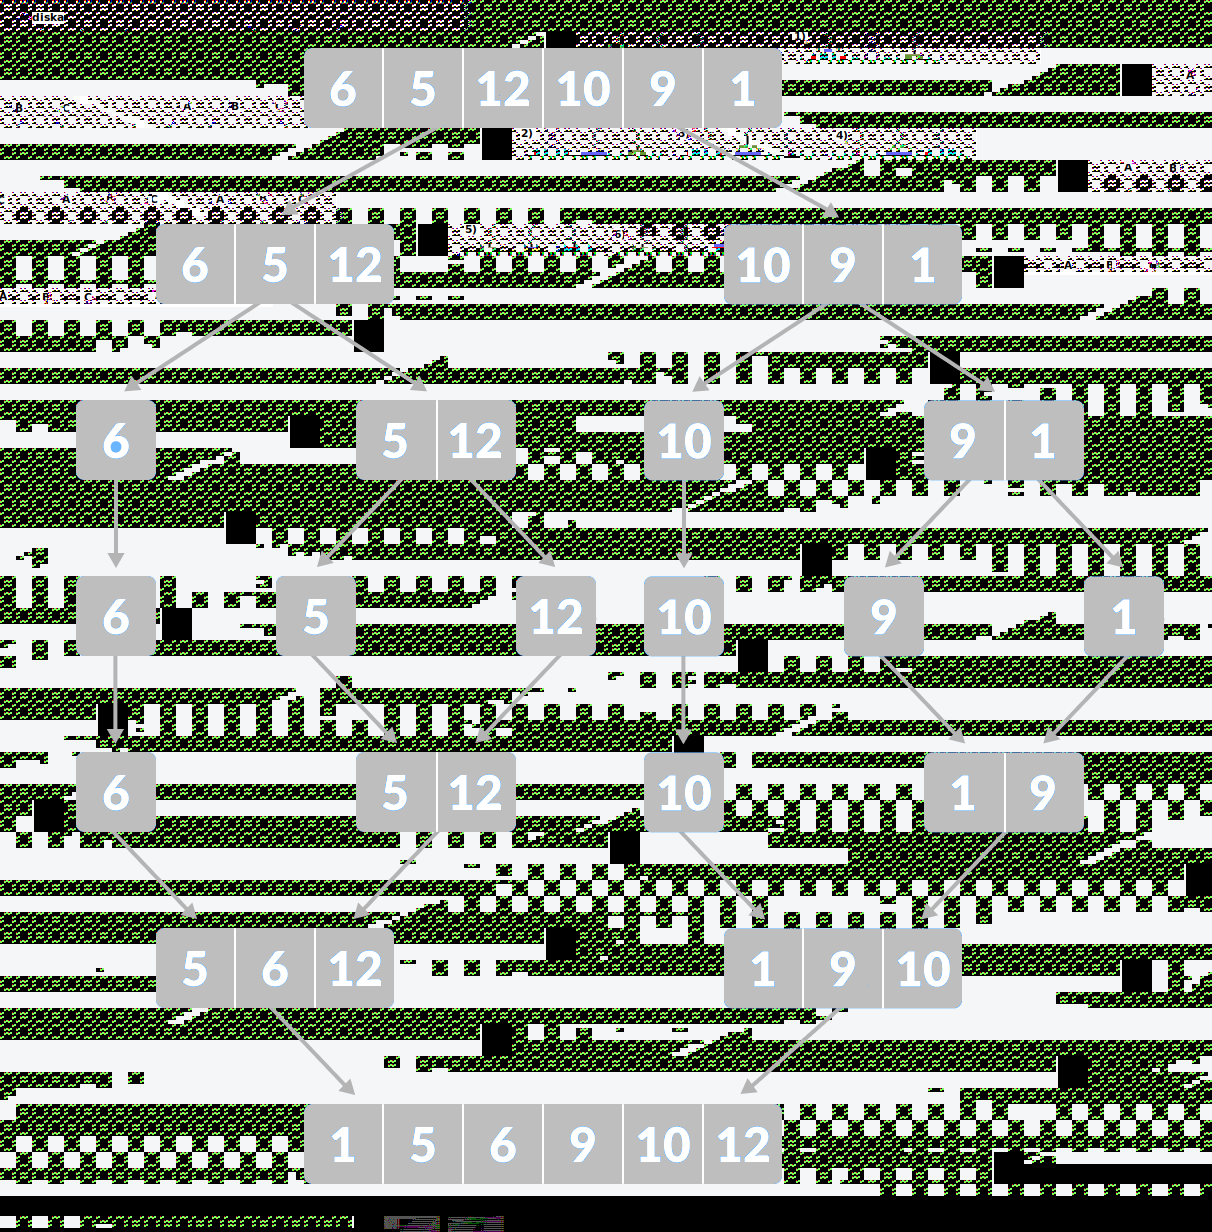
\includegraphics[width=200pt,height=150pt]{slike/merge-sort-example.png}
 	\label{fig:merge-sort}
 	\caption{Sortiranje spajanjem pomoću podijeli pa zavladaj paradigme: koraci}
 \end{figure}

\begin{example}

\textbf{\textit{Množenje cijelih brojeva}}. Za  množenje dva $n$-cifrena broja, metodom koji se uči u nižim razredima osnovne škole, množeći cifru po cifru, zahtijeva se vrijeme izvršavanja od $O(n^2)$.  Konstruisati algoritam zasnovan na paradigmi podijeli pa zavladaj za problem množenje dva broja. 
\end{example}
\begin{solution}
 
 
 Jednostavnosti radi, smatramo da su u ulazu binarni brojevi sa istim brojem cifara.
Pokušajmo sa alternativnom metodom koja će voditi paradigmi zavadi pa vladaj.  Napišimo svaki od brojeva u obliku: $x= x_1 2^{n/2} + x_2, y= y_1 2^{n/2} + y_2$.
Tada je 
$$ xy = (x_1 2^{n/2} + x_2) \cdot (y_1 2^{n/2} + y_2) = x_1 y_1 2^n + (x_1 y_2 + y_1 x_2)2^{n/2} + x_2y_2.$$
Dakle, da bismo izračunali proizvod dva (binarna) broja sa $n$ cifara, treba da izračunamo proizvod $q=4$ broja sa po $n/2$ cifara. Stoga, kompleksnost u ovom sljučaju je i dalje $O(n^{\log_2 4}) = O(n^2)$. Da bismo ubrzali algoritam,   uradimo sljedeće operacije u datom redoslijedu:
\begin{itemize}
	\item Izračunajmo $x_1y_1$ i $x_2 y_2$.
	\item Izračunajmo $(x_1 + x_2 ) \cdot (y_1 + y_2) = x_1y_1 + x_1y_2 + x_2 y_1 + x_2 y_2$.
	\item Iz prethodnog izraza izvucimo vrijednost $x_1 y_2 + x_2 y_1$.
\end{itemize}
Iz master teoreme, slijedi da je sada kompleksnost algoritma jednaka $O(n^{\log_2 3})$.
\end{solution}

\section{Algoritamska paradigma vraćanja unazad }

  \textit{Vraćanje unazad} je algoritamska tehnika za rekurzivno rješavanje problema postepenom izgradnjom  rješenja, dio po dio, uklanjajući ona (parcijalna) rješenja koja ne zadovoljavaju ograničenja problema, momentalno nakon dodavanja nove komponente (odnosi se na vrijeme koje je proteklo do dostizanja bilo kojeg nivoa stabla pretraživanja). Za ovu paradigmu se može reći da je ona  poboljšanje pristupa grube sile.
  
  U osnovi,   traži  se  rješenje problema među svim dostupnim opcijama. U početku krećemo od jedne moguće opcije i ako se problem može riješiti tom opcijom, vraćamo dato rješenje. U suprotnom vraćamo se unazad, birajući drugu opciju među preostalim   opcijama. Slučaj u kojem  niti jedna od opcija ne daje rješenje rezultira scenarijem da se neće naći nikakvo rješenje za  određeni problem.  Vraćanje unazad predstavlja rekurzivni pristup jer se proces pronalaska rješenja iz različitih dostupnih opcija rekurzivno ponavlja, sve dok se ne nađe rješenje problema ili dok se dođe do konačnog stanja.
  
  
   Tehnika vraćanja unazad u svakom koraku eliminiše one izbore koji ne mogu dati rješenje i nastavlja   sa onim izborima koji imaju potencijal da odvedu do rješenja. Algoritmi vraćanja unatrag su generalno eksponencijalni i  vremenski i prostorno te se ne preporučuju za rješavanje teških problema.  
    
    Postavlja se pitanje kako prepoznati da se neki problem može riješiti pomoću ove algoritamske paradigme. Dakle, osnovna ideja je da se rješenja problema mogu konstruisati inkrementalno, dodavanjem jedne kompomente za drugom u svakom koraku u postojeće (parcijalno) rješenje, dok se ne dobije rješenje problema ili ne utvrdi da se tim izborom komponenete, nikada neće dobiti validno rješenje (nakon čega se pretraga vraća nazad, pretražujući druge opcije). Prevedeno na jezik rješavanja podproblema, algoritamska paradigma vraćanja unazad rješava sve podprobleme jedan za drugim, kako bi  došla do najboljeg mogućeg rješenja. 
    
    Pseudokod paradigme varaćanja unazad je dat Algoritmom~\ref{alg:backtrack}. 
    
    \begin{algorithm}
    	\begin{algorithmic}[1]
    		\Procedure{Backtrack}{$x$}
    		   \If{$x$ nije rješenje}
    		        \State return \textbf{false}
    		   \EndIf
    		  \If{$x$ je novo rješenje}
    		     \State dodaj $x$ u listu rješenja
    		  \EndIf
    		 \For{svaku moguću opciju $e$}
    		      \State \textsc{Backtrack}(proširi $x$ sa $e$)
    		  \EndFor
    		\EndProcedure
    	\end{algorithmic}

        \caption{Paradigma vraćanja unazad. }        \label{alg:backtrack}
    \end{algorithm}
    
    Napomenimo da je implementacija ovog algoritma vezana za konstruisanje stabla odluke, koje se češće naziva \textit{stablo stanja} (eng. \textit{state-space tree}). U okviru ovog kursa ne ulazimo u ovu notaciju, nego bez previše formalizma pokušavamo objasniti rad osnovnih algoritamskih paradigmi i način rješavanja problema pomoću svake od njih.    
    
    %https://www.programiz.com/dsa/backtracking-algorithm ==> primjer 1...
    
    \begin{example}
    	\textbf{\emph{Problem N kraljica}}.  Neka je data šahovska ploča dimenzije $N\times N$. Smjestiti $N $ kraljica na šahovsku ploču tako da se nikoje dvije kraljice međusobno ne napadaju.  Korisiti algoritam vraćanja unazad. 
    \end{example}

\begin{solution}
           
      Pogledajmo problem 8 kraljica, te jedno njeno rješenje dato na sljedećoj slici.  
      \begin{figure}[H]
      	\centering
      	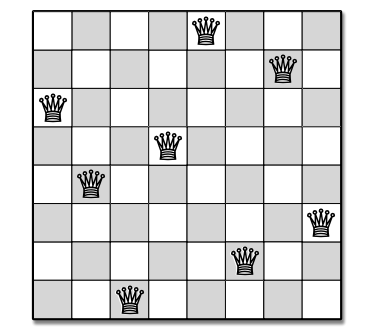
\includegraphics[width=200pt,height=180pt]{slike/n-queen-problem.png}
       
  \end{figure}

Jasno je da se po jedna kraljica smiješta u svakom redu šahovske ploče. Pozicija kraljice u $i$-tom redu je određena brojem kolone u kojoj je ta kraljica postavljena. U prevodu, svako rješenje koje odgovara poziciji kraljica na ploči možemo kodirati nizom \emph{niz} dužine $N$, gdje se na poziciji $i$ nalazi broj kolone u $i$-tom redu u kojoj je smještena kraljica. Konkretno, rješenje (pozicije kraljica)  na prethodnoj slici kodirano je nizom $[5, 7, 1, 4, 2, 8, 6, 3]$. 

Algoritam vraćanja unazad kreće od inicijalno prazne ploče i u svakom koraku nastoji dodati kraljicu u sljedeći (prazni) red. Dakle, kreće se od praznog rješenja, u koji se dodaje novi element   koji odgovara poziciji kraljice sljedećeg (nepopunjenog) reda. Stoga, pri dodavanju nove kraljice u rješenje \emph{niz}, ispitujemo da li pozicije kraljica u (produženom) rješenju  zadovoljavaju uslove zadatka (ne  postoje dvije kraljice koje napadaju jedna drugu). U slučaju da postoji konflikt između nekih kraljica, algoritam se vraća unazad na rješenje \emph{niz} prije dodavanja posljednje dodane kraljice, i razmatra nove pozicije za dodavanje kraljice u tom redu -- tj. za proširivanje trenutnog rješenja.  Ovaj proces se ponavlja sve dok se ne nađe prvo rješenje dužine $N$ koje zadovoljava uslove zadatka (tj. popune se svi redovi na ploči sa kraljicama koje se međusobno ne napadaju), ili se ustanovi da takvo rješenje ne postoji. 

   
Implementacija u Pajtonu koja rješava ovaj problem je data narednim k\^odom. 

\begin{minted}{python}
	
   def NQueens(niz, N):
       if len(niz) == N: # kompletno rješenje
               return niz
       else:
              for i in range(N):
                  niz = niz + [i]
                  if not valid(niz): #backtrack ako nije 
                     NQueens(niz + [i])

N = 8
sol = NQueens([], N)       
if sol != None:
   print("Rješenje je: ", sol)
else:
   print("Nema rješenja") #npr. za N=3
   
\end{minted}
%%https://codeahoy.com/learn/recursion/ch10/
\begin{figure}
	\centering
	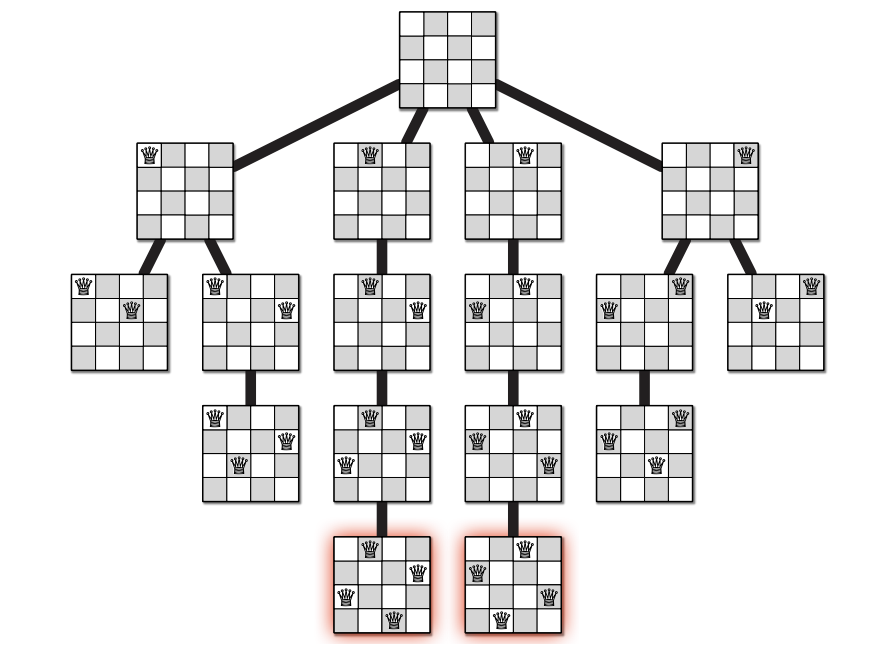
\includegraphics[width=320pt, height=250pt]{slike/recursion-tree-backtracking-n-queens.png}
	\caption{Primjer stabla stanja formiranog algoritmom vraćanja unazad za problem 4 kraljice}
\end{figure}

Napomenimo da ovdje nismo prikazali implementaciju funkcije \textit{valid}(), koja vraća \textit{True} ako je pozicija kraljica  validna, u protivnom vraća \textit{False}. Ovo ostavljamo čitaocu kao zadatak za vježbanje. 


\end{solution}


    
 % Što se tiče problema koje ova paradigma rješava, dijelimo ih na tri tipa:
  %\begin{itemize}
  %	\item   \textit{Problem odlučivanja} -- U ovom slučaju tražimo izvodljivo rješenje.
  %	\item   \textit{Problem optimizacije} – U ovome tražimo najbolje rješenje.
  %	\item   \textit{Problem enumeracije} – U ovome nalazimo sva izvodljiva rješenja.
  %\end{itemize}


%https://codeahoy.com/learn/recursion/ch11/: THE SUM OF 4 SQUARES:

\begin{example}
	\textit{Problem sume 4 kvadrata}. Lagranžova teorema o 4 kvadrata kaže da se svaki prirodni broj može napisati kao zbir četiri broja koji su kvadrati nekih brojeva. Neka je dat broj $n$. Naći četiri kvadratna broja koji u zbiru daju broj $n$ pomoću algoritma vraćanja unazad. \\
	Npr. za $n=2000$, vrijedi $1764 + 196 + 36 + 4 = 2000. $
\end{example}

\begin{solution}
	Rješenje problema predstavlja četvorka $sol = (a, b, c, d)$ prirodnih brojeva, tako da je $a^2 + b^2 + c^2 + d^2 = n$. Ideja rekurzije je odabrati svaki  od brojeva jedan po jedan, dok ne dobijemo četvorku koja odgovara uslovima zadatka. Svaki put kada dodamo novi broj $x$ u rješenje \emph{sol}, naredni rekurivni poziv ispituje trenutno zbir kvadrata brojeva u proširenom rješenju \emph{sol}. Ako ono prelazi $n$, algoritam vrši vraćanje unazad i bira novog kandidata za proširivanje rješenja. 
	
 Implementacija algoritma vraćanja unazad za ovaj problem je dat narednim k\^odom.
 
 \begin{minted}{python}
 	  
from math import sqrt, pow

def FourSquareSum(sol):
	sum = 0
	for s in sol:
		sum += pow(s, 2)
	return int(sum)

def FourSumSquares(sol, n):
	if len(sol) == 4:
		if FourSquareSum(sol) == n:
			print(sol)
	else:
		for i in range(1, int(sqrt(n))+2):
			solI = sol + [i]
			sum_sol_i = FourSquareSum(solI)
			if sum_sol_i <= n-(4-len(solI)): # else backtrack  
				FourSumSquares(solI, n) 
# poziv metode
FourSumSquares([], 20)
 \end{minted}
	
	Kao što primijećujemo u prethodnom kodu, ako je \emph{sol} kardinalnosti 4, i ako je zbir kvadrata njegovih elemenata jednak $n$, ispisujemo \emph{sol} kao rješenje. U protivnom, ako je $|sol|<4$, (parcijalno) rješenje \emph{sol} proširujemo ubacujući naredni broj (varijabla $i\in \{1, \ldots, \lfloor\sqrt{n} \rfloor + 1 \}$), dobijajući niz \emph{solI}.  Ako je zbir kvadrata elemenata iz \emph{sol} veći od $n-(4 - |solI|)$, ovakva ekstenzija nikada neće voditi ka rješenju koje zadovoljava uslove zadatka, pa pretraga ide unazad, rekurzivno, provjeravajući druge kandidate za proširenje trenutnog rješenja \emph{sol}. Na početku, rješenje \emph{sol} je predstavljeno prazanim nizom.
	 
\end{solution}
 
 
\section{Pohlepni algoritmi}
 % https://www.programiz.com/dsa/greedy-algorithm
\textit{Pohlepni algoritam} je pristup rješavanju problema odabirom najbolje dostupne opcije u datom trenutku za trenutno rješenje u koristeći neki (pohlepni, intuitivni) kriterijum. Pristup ne brine da li će lokalno najbolji odabir uticati ili ne na optimalni rezultat. Algoritam nikada ne poništava raniju odluku čak i u slučaju da je izbor pogrešan. Upravo zbog toga se ovom algoritamskom paradigmom generalno ne može  garantovati nalazak optimalnog rješenja. Dakle, uvijek se traži najbolji lokalni izbor očekujući da će ta odluks voditi   najboljem globalnom rezultatu. U principu, ova paradigma pripada   pristupu \textit{odozgo prema dolje} (eng. \textit{top-down approach}). 

U neformalnom smislu, pohlepni algoritam je algoritam koji počinje jednostavnim, nekompletnim, tj. parcijalnim rješenjem (teškog) problema, a zatim iterativno traži najbolji način za poboljšanje rješenja proširujući ga iterativno, dok ono ne postane kompletno (neproširivo). Pseudokod ove algoritamske paradigme je dat Algoritmom~\ref{alg:greedy-algorithm}. 

Ulaz u algoritam su problem $\mathcal{P}$, instanca problema, te pohlepna funkcija $g$.  Algoritam kreće od nekog, obično praznog, parcijalnog rješenja koje se kroz iteracije nastoji proširiti najboljim mogućim odlukama (komponentama). U svakoj iteraciji izvršava se sljedeće:
 \begin{itemize}
 	\item Za trenutno rješenje $x$, izračunavaju se komponente koje dopustivo (u odnosu na ograničenja problema) proširuju $x$;
 	\item Među svim takvim komponentama, bira se ono koje (naizgled) najviše doprinosi kvalitetu krajnjeg rješenja; ova odluka se donosi na osnovu pohepne funkcije $g$, koja se još naziva i \textit{heuristička} funkcija. 
 	\item Proširimo rješenje sa najboljom komponentom rješenja.
 \end{itemize}
Ovaj proces se izvršava sve dok je skup komponenti koje dopustivo proširuju trenutno rješenje neprazan. Nakon prekida, vraćamo dobijeno rješenje.

 %%Proces se ponavlja sve do nekog uslova zaustavljanja.

\begin{algorithm}
	\begin{algorithmic}[1]
		\State \textbf{Ulaz:}   instanca nekog problema $\mathcal{P}$, pohlepna funkcija $g$
		\State \textbf{Izlaz}: (aproksimativno) rješenje instance problema $\mathcal{P}$
		\State $x\gets$ inicijalno parcijalno rješenje problema $\mathcal{P}$
		\State $\mathcal{C}\gets$ odredi komponente rješenja koje dopustivo proširuju rješenje $x$
		\While{$\mathcal{C} \neq \emptyset$}
		    \State $e \gets$ odaberi lokalno najbolju komponentu iz $\mathcal{C}$ u odnosu na pohlepnu funkciju $g$
		    \State Proširi $x$ sa $e$
		     \State $\mathcal{C}\gets$ odredi komponente rješenja u odnosu na prošireno rješenje $x$
		\EndWhile
		%\If{$x$ je dopustivo}
		   \State \textbf{return} $x$
		%\Else
		 %   \State Poruka da (dopustivo) rješenje nije nađeno
		%\EndIf
	\end{algorithmic}

    \caption{Shema paradigme pohlepnih algoritama.}    \label{alg:greedy-algorithm}
\end{algorithm}

Dakle, da bimo primijenili pohlepni pristup u rješavanju problema, potrebno je definisati: ($i$) skup komponenti rješenja; ($ii$) strukturu parcijalnog rješenja; ($ii$) pohlepnu funkciju koja računa kvalitet komponente koja može proširiti postojeće parcijalno rješenje. 



Ovu paradigmu koristimo kada je potrebno dobiti rješenje razumnog kvaliteta   u relativno kratkom vremenskom intervalu, na jeftin način (kodirajući relativno brzo). Ovo je često jedna od prvih tehnika koja se primijenjuje u rješavanju teških 
problema.  Ovi algoritmi se takođe koriste u svrhu dobijanja početnog rješenja koje se zatim  poboljšava naprednijim tehnikama. U osnovi, ova paradigma nam nudi dobru polaznu osnovu da ``opipamo'' problem, da se osjeti  koliko je on težak, te da se dobije na uvid koliko heurističke, konstruktibilne (aproksimativne) metode mogu biti efikasne za rješavanje takvih problema.

U nastavku navodimo nekoliko primjena pohelpnih algoritama u rješavanju raznih tipova (kombinatornih) problema. 

\subsection{Problem razmjene novca}

\begin{example}
 Imamo  $X$ KM-ova. Na rapolaganju su apoeni od $x_1, x_2, \ldots , x_k$ KM-ova, negoraničene količine. Pretpostavimo da su $X, x_i, i=1,\ldots, n$ prirodni brojevi.

Kako razmijeniti $X$ KM-ova tako da dobijemo što manji broj
novčanica? Rješiti zadatak pomoću paradigme pohlepnih algoritama.
\end{example}

\begin{solution}
	 Definišimo rješenje problema i njegovu strukturu. Bilo koja $k$-torka $(p_1, p_2, \ldots , p_k )$, gdje je $p_i$ broj
	 apoena novčanice od $x_i$ KM-ova tako da je $\sum_i p_i = X$
	 (razmjenjena je količina od $X$ KM-ova) prestavlja (dopustivo) rješenje. 
	 Parcijalno rješenje problema je bilo koja $s$-torka $(p_1, p_2, \ldots , p_s )$ za koju je $\sum_i^s p_i \leq X, s \leq k$.  Ovakvo rješenje se može nadopuniti do dopustovog. \\ 
	 
	 Konstruišimo sada pohlepnu funkciju. Ideja je da prvo razmatramo novčanice najvećeg mogućeg apoena koji je manji od $X$. Uzmemo takvih novčanica koliko možemo, ali da ne pređemo vrijednost od $X$. Od preostalog iznosa $X'$ koji treba da bude razmijenjen, uzmemo onoliko novčanica maksimalnog apoena, koji je manji od $X'$, koliko god je to  moguće. Ovaj proces nastavimo, dok ne dobijemo dopustivo rješenje. 
	 
	 Prema tome, prvo sortiramo vrijednosti apoena od najvećeg do najmanjeg. Pretpostavimo bez smanjenja opštosti da je  početni redoslijed apoena $x_1, \ldots, x_k$ dat u sortiranom poretku. Pohlepna funkcija od trenutnog parcijalnog rješenja $s_{partial}=(p_1, \ldots, p_s), s \leq k$ nalazi najmanji indeks apoena $i$ koji je veći od $s$, a da je pri tome $x_i \leq X'= X - \sum_i^s p_i x_i$. Tada je novo prošireno parcijalno rješenje jednako 
	 $$s'_{partial}=(p_1, \ldots, p_s,{0,\ldots, 0}, \underbrace{\lfloor X'/x_i \rfloor}_{p_i} ).$$ 
	 Algoritam se završava kada razmotrimo sve apoene, ili prije toga, kada algoritam nađe rješenje.  K\^od algoritma   je dat u nastavku.
	 \begin{minted}{python}
	 def razmijeni(P, X):
	 	rjesenje = []
	 	i = 0
	 	usitnjeno = 0
	 	brojNovcanica = 0
	 	sortApoeni = sort(P) # sort apoene opadajuće
	 	while i <  n and usitnjeno < X :
	 		k = (X - usitnjeno) // P[i]  #br. novcanica sortApoeni[i] ide u razmjenu
	 		if k > 0:
	 			usitnjeno = usitnjeno + k * sortApoeni[i]
	 			brojNovcanica = brojNovcanica + k
	 		i = i + 1
	 	if usitnjeno == X:
	 		return brojNovcanica
	 	else:
	 		return -1 # ne može se usitniti
	 \end{minted} 
\end{solution}

\textit{Kompleksnost algoritma}. Sortiranje algoritma zahtjeva vrijeme od $O(n \log n)$. Dalje, glavna petlja se izvršava u $O(n)$ vremenu, odakle slijedi da je ukupno vrijeme izvršavanja algoritma jednako $O(n \log n)$, što je, svakako, polinomijalno.  Naopmenimo da ovakvom strategijom garantujemo nalazak optimalnog rješenja problema (ili utvrđujemo da rješenje ne postoji). 


\subsection{Dijeljeni problem ruksaka}
\begin{example}
  Ovaj problem je relaksirana verzija problema ruksaka, obrađen u prethodnim sekcijama. Odluka da li uzeti (cio)  proizvod ili ne i staviti u ruksak se relaksira na to da se bilo koji (razlomljeni) dio proizoda može uzeti i staviti u ruksak. Zamislimo da je u pitanju proizvod kao što je šećer ili ulje koji (teorijski) može da se dijeli na bilo koji razlomljeni  (realni) dio.  \\
  
   Zadatak je odabrati proizvode (dijelove proizvoda) i staviti u ruksak, tako da je profit maksimalan, ali da se poštuje ograničenje za kapacitet  ruksaka. Koristiti paradigmu pohlepnih algoritama. 
\end{example}

\begin{solution}
	Posmatrajmo primjer instance: $$n = 3, w = [10, 20, 30], p = [60, 100, 120],$$  a 
	kapacitet $C = 50$.  Rješenje ove konkretne instance je uzeti prvi i drugi proizvod u potupnosti (svih 10 i
	20(kg)), dok uzimamo 2/3 trećeg proizvoda (20). Kapacitet ruksaka je zadovoljen,
	a vrijednost proizvoda u ruksaku je jednaka $60 + 100 + 2/3 \cdot  120
	= 240$. \\
	
    \textit{Rješenje i struktura problema}.  Rješenje $c = \{c_1,\ldots, c_n\}$, gdje je $0 \leq c_i \leq 1$ dio uzetog
    proizvoda $i$ koji je stavljen u ruksak, a pri tome je zadovoljen  uslov o nepremašivanju kapaciteta ruksaka u vrijednosti   $C$.
    
    \textit{Parcijalno rješenje i komponente rješenja}. Parcijalno rješenje $c = \{ c_{i_1}, \ldots, c_{i_k}  \}$, pri čemu je $i_s \in [n],  i_s \neq i_r, s\neq r,   k \leq n$, a kapacitet ruksaka je zadovoljen. 
    Komponente rješenje u odnosu na parcijalno rješenje $s$ su svi oni proizvodi $C_s = [n] \setminus \{  {i_1}, \ldots, {i_k} \}$ koji se trenutno ne nalaze   u ruksaku. Proširenje parcijalnog rješenja podrazumijeva operaciju dodavanja  količine $c_r>0$ onog proizvoda $r \in C_s$, tako da proširivanjem rješenja $s$ ovom komponentom ne narušavamo kapacitet ruksaka. 
    
    \textit{Pohlepna funkcija}.  Razmotrimo sljedeću razumnu strategiju. Favorizujmo proizvode koji imaju veću cijenu po (jednici) težine, tj. kojima je količnik  $\frac{c_i}{w_i}$ veći u odnosu na ostale. Sortirajmo proizvode po ovom kriterijumu. Neka je, bez smanjenja opštosti, sortirani redosljed proizvoda po ovom kriterijumu dat sa (indeksima) $1,2, \ldots, n$.   \\
    
    
    Dodajmo dio $c_1$ proizvoda indekiranim sa $1$ koliko god je to moguće (maksimalno 1) u odnosu na kapacitet ruksaka. Ako je  $c_1 = 0$, to znači da je kapacitet ruksaka zadovoljen, pretraga se završava. Inače, nastavimo istom strategijom, ažurirajući preostalo stanje ruksaka koji treba da se popuni, a zatim posmatrajući naredni proizvod (sa indeksom 2). Potom određujemo maksimalni udio proizvoda $c_2\geq 0$ koji   (dopustivo) proširuje trenutno  parcijalno rješenje, itd. Petpostavimo da smo istom strategijom generisali rješenje $s = \{ c_{1}, \ldots, c_{k}\}$. %, i_1< \ldots < i_k$.
     Slično, posmatramo naredni proizvod sa indeksom $i =  k+1$, te izračunamo udio tog proizvoda $c_{i}$ kojeg ćemo ubaciti u ruksak, tj. proširiti rješenje $s$. Ako je $c_i = 0$, pretraga se završava. U protivnom, dodajemo komponentu u trenutno parcijalno rješenje, uz ažuriranje stanja o kapacitetu ruksaka koji je preostao za popunjavanje. Pretraga traje sve dok ne popunimo ruksak ili ne razmotrimo sve proizvode.  
    
   Implementacija algoritma je data naredim k\^odom. 
   
   \begin{minted}{python}
  def fraction(i):
  	return P[i]/ W[i]
  
  def fraction_knapsack():
  
  	products = [i for i in range(len(W))] #lsit of prods
  	products.sort(key = fraction, reverse=True)
  	#print(products)
  	current_C = C
  	sol = []
  	parts = []
  
  	for i in products:
  
  		part = min(current_C / W[i], 1)
  
  		if part > 0:
  			sol.append(i)
  			parts.append(part)
  			current_C -= part * W[i]
  
  		else: # knapsack filled
  			return sol, parts
    return sol, parts
    #instanca: 
    W = [10, 20, 30]
    P = [60, 100, 120]
    C = 50
    sol, parts = fraction_knapsack()
    print(sol, " parts: ", parts)
  
   \end{minted}

\textit{Kompleksnost algoritma}.  Najviše vremena je utrošeno na sortiranje proizvoda, što iznosi $O(n \log n)$ vremena. Dalje, u glavnoj petlji, koja se vrti najviše $n$ puta,  svaka iteracija se izvršava u konstantnom vremenu. Dakle, vrijeme izvršavanja petlje je $O(n)$. Prema tome, algoritam se izvršava u $O(n \log n)$ vremenu.

Napomenimo da ovaj algoritam takođe garantuje nalazak optimalnog rješenja. 
\end{solution}


\begin{example} \textbf{Problem pokrivanja skupa}. Neka je dat skup $X$ i podskup njegove familije podskupova $\mathcal{F} \subseteq P(x)$, pri čemu je
	$\cup_{f \in F} f = X$.
	
	Naći podskup $S \subseteq F$ minimalne kardinalnosti $|S|$, tako da je 
  $\cup_{s \in S} s = X$. Problem riješiti uz pomoć paradigme pohlepnih algoritama. 
	
\end{example}

\begin{solution}
	
	Neka je data instanca problema $X = \{1, 2, 3, 4, 5\},$ te $
	\mathcal{F} = \{\{1, 2, 3\}, \{1, 4\}, \{2, 4, 5\}, \{2, 3\}, \{4, 5\}, \{1, 5\}\}$. 
	Rješenje problema je dato sa $S =$ $ \{\{1, 2, 3\}, \{2, 4, 5\}\}$. Njegova kardinalnost je $|S| = 2$.
	
	Ovaj problem ima konkretnu praktičnu primjenu u odabiru minimalnog broja ljudi u komisiju, a da komisija bude kompetentna u svakoj od (traženih) oblasti. Konstruišimo sada algoritam. \\
\textit{Rješenje i struktura rješenja.} Skup (skupova) $S \subseteq \mathcal{F}$ je rješenje problema ako unijom elemenata svih skupova iz $S$ dobijamo skup $X$. 

\textit{Parcijalno rješenje i komponenta rješenja}. Pod parcijalnim rješenjem ovog problema podrazumijevamo bilo koji (pod)skup $S \subseteq \mathcal{F}$ koji ne mora obavezno zadovoljavati uslov o pokrivanju skupa $X$.  Komponenta rješenja $S$ je bilo koji skup iz $C \in \mathcal{F} \setminus S $, dok proširenje rješenja $S$ komponentom rješenja $C$ podrazumijeva operaciju unije, tj. $S' = S \cup \{ C \} $.

\textit{Pohlepna funkcija}. Neka je $S$ parcijalno rješenje i neka ono pokriva $X_S' \subseteq X$ elemenata. Intuitivno, bolja opcija podrazumijeva biranje kompomente rješenja $C$ koja u presjeku sa skupom $X \setminus X_S'$ ima više elemanta  nego neki drugi $C'$ sa manjim takvim brojem. Razlog je taj što nastojimo pokriti što više skupa $X$ u što manjem broju koraka pohlepnog algoritma. U simboličnom zapisu, pohlepna funkcija ima sljedeći oblik
$$ g(S, C) = | C \cap ( X \setminus X'_S) |,$$
dok biramo element $C^*$ tako da 
$$ C^* \gets argmax \{ g(s, C') \mid C'\in \mathcal{F} \setminus S\} $$
kao element koji će proširiti parcijalno rješenje $S$ u datoj iteraciji.


Algoritam u svakom koraku bira skup $C^*\in \mathcal{F}$ u odnosu na pohlepnu funkciju $g$  i dodaje ga u parcijalno rješenje dok god   rješenje ne pokrije čitav skup $X$, nakon čega se algoritam prekida. Napomenimo da se umjesto kompletnih skupova koji se čuvaju u rješenju $S$, mogu čuvati pozicije (indeksi) skupova iz $\mathcal{F}$ koji pripadaju rješenju $S$. 

Implementacija algoritma  je data u nastavku sljedećim k\^odom.

\begin{minted}{python}
	def g(X_S, C):
		return len((X.difference(X_S)).intersection(C))
	def cover_X():
		X_S = set(())
		S = [] # solution
	
		while(X_S != X):
			C_star = istar = None
			g_best = 0
	
			for i in range(len(F)):# iteration best-next
				if i  not  in S: 
					g_i = g(X_S, F[i])
					if g_best < g_i:
						g_best = g_i
						i_star = i
	
			X_S = X_S.union(F[i_star]) #update cover
			S.append(i_star)
		return  S            
	
	#instanca: 
	X = {1, 2, 3, 4, 5}
	F = [{1, 2, 3}, {1, 4}, {2, 4, 5}, {2, 3}, {4, 5}, {1, 5}]
	sol = []
	C = 50
	sol = cover_X()
	print(sol)
	
\end{minted}

\textit{Kompleksnost algoritma}. Glavna \texttt{while}-petlja se izvršava u najviše $n$ iteracija. Dalje, U unutrašnjoj \texttt{for}-petlji, koja se izvršava  $ |\mathcal{F}|$ puta, najskuplja operacija je pozivanje \texttt{g} funkcije, koja se izvršava u   najviše linearnom vremenu, tj. pripada $O(n)$. Dakle, kompleksnost čitave \texttt{for} petlje je $O(n \cdot  |\mathcal{F} |)$. Dakle, kompleksnost algoritma je $O(n^2 \cdot  |\mathcal{F} |)$. Prema tome, efikasnost algoritma najviše zavisi od veličine skupa $\mathcal{F}$. 

Napomenimo da ovako dizajniran algoritam ne garantuje nalazak optimalnog rješenja  kao u prethodna dva problema. 


  Uzmimo npr. instancu $X= \{1, 2, 3, 4, 5, 6\}$, te $$\mathcal{F}= \{\{1,2\}, \{3, 4\}, \{4, 5\}, \{3, 6\}, \{5\}, \{6\} \}.$$   
  Prva iteracija u algoritmu će uzeti, recimo, prvi skup $\{1, 2\}$ u parcijalno rješenje. Dalje, naredna iteracija uzima skup $\{3, 4\}$. Nakon toga, bira se $\{4, 5\}$, pa $\{6\}$. Dakle, konačno rješenje je kardinalnosti 4. Međutim, to očigledno nije optimalno rječenje. Optimalno rješenje   je veličine 3 i dato je sa $\{ \{1, 2\}, \{3, 6\}, \{4,5\}\}$.  
	 
\end{solution}

\begin{example}  \textbf{\textit{Problem sekvencijalnog raspoređivanja poslova}}. Dat je skup  poslova, gdje svaki posao ima dozvoljeno krajnje
	vrijeme završetka (eng. \textit{deadline}) i odgovarajući profit, ako  posao bude završen 
	prije tog vremena. Pretpostavimo da je za izvršavanje svakog posla  potrebno identično (jedinično)
	vrijeme. Startno vrijeme za izvršavanje svih poslova je isto za sve poslove (pretpostavljamo da kreće od 0). \\
	
	  Maksimizovati ukupni profit, ako samo jedan
	posao može da bude izvršen u svakoj jedinici vremena. Riješiti problem pomoću paradigme pohlepnih algoritma. 
\end{example} 

\begin{solution}
	Posmatrajmo primjer instance problema, data sljedećom tabelom.
\begin{center}
 
 
	\begin{tabular}{ccc }
	 \centering
	Posao (ID) & Krajnji rok (Dedlajn) & Profit \\ \hline \hline
	$1$	&	4	&	20 \\
	$2$	&	1	&	10\\
	$3$	&	1	&	40\\
	$4$	&	1	&	30\\ \hline
	\end{tabular}
\end{center}

Otimalan odabir poslova u slučaju ove instance je: $\{3, 1\}$, sa profitom od 60. 

Posmatrajmo narednu instancu problema.  
\begin{center}
	
	
	\begin{tabular}{ccc }
		\centering
		Posao (ID) & Krajnji rok (Dedlajn) & Profit \\ \hline \hline
		$1$	&	2	&	100 \\
		$2$	&	1	&	19\\
		$3$	&	2	&	27\\
		$4$	&	1	&	25\\  
	 $5$	&	3	&	15\\   \hline
	\end{tabular}
\end{center}
	
\end{solution}

Rješenje za ovu instancu je odabir poslova iz skupa $\{3, 1,5 \}$ redom kako su i navedeni. Profit ovog rješenja je 142. 


Prva ideja za rješavanje ovog problema je koristiti potpunu enumeraciju: generisati sve podskupove
skupa poslova te za svaki od njih provjeriti dopustivost i na taj način pratiti  
maksimalni profit. Međutim, razmotrimo  tehniku pohlepnih algoritama. 

\textit{Rješenje i struktura rješenja}. Svaki podskup $I_s$ skupa svih poslova $I=\{1,\ldots, n\}$ koji zadovoljava uslove zadatka (da se svi mogu izvršiti u okviru njihovog krajnjeg vremena izvršavanja, te nijedan se ne izvršava paralelno sa drugim),  predstavlja rješenje problema. Dalje, struktura rješenja može da bude predstavljena strukturom podataka koja odgovara skupu. 

\textit{Parcijalno rješenje i njegovo proširenje}.  Parcijalno rješenje je bilo koji podskup skupa poslova koji zadovoljava uslove zadatka. Ostatak poslova, koji može da se doda postojećem skupu poslova, a pri tome da ne naruši uslove zadatka, pripada skupu komponenti rješenja koje proširuju dato (parcijalno) rješenje. 

\textit{Pohlepna funkcija}. Za parcijalno rješenje $I_s$, odabrati komponentu rješenja (posao) $i \in I\setminus I_s$ sa maksimalnim profitom koji proširuje $I_s$ na dopustiv način (uslovi zadatka su ispunjeni). Taj posao se, pri tome, smiješta u prvi slobodan (jedinični) interval u kojem se izvršava. 


\textit{Algoritam}. Sortirajmo poslove u odnosu na njihov profit (opadajuće). Bez smanjenja opštosti, pretpostavimo da su oni dati u poretku $\{1, 2, \ldots, n\}$. U provoj iteraciji dodajemo posao 1 maksimalnog profita u parcijalno rješenje $I_s$, koje je inicijalno prazno.  Dalje, pretpostavimo da smo u $i$-toj iteraciji generisali parcijalno rješenje $I_s$. Tada, u narednoj iteraciji razmatramo posao indeksiran sa $i+1$. Moguća su dva scenarija.

\begin{itemize}
	\item Posao sa indeksom $i+1$ ne može da proširi trenutno parcijalno rješenje $I_s$; u tom slučaju idemo na naredni posao ($i+2$);
	\item Posao sa indeksom $i+1$ može da bude dodan u $I_s$. U tom slučaju, nalazimo prvi slobodan jedinični interval u kojem taj posao može da bude izvršen, u odnosu na već raspoređene poslove u trenutnom rješenju $I_s$.  
\end{itemize} 

Algoritam se izvršava sve dok se ne iteriše kroz sve poslove, nakon čega se vraća konačno rješenje. Implementacija algoritma je data sljedećim k\^odom. 
 
 \begin{minted}{python}
 
 def ProfitSort(i):
 	return Profit[i]
 
 # možemo li dodati i-ti proizvod ili ne (-1) u I_s
 def find_next_interval(I_s_covered, i):
 
 	for index, covered in enumerate(I_s_covered):
 		if index >= Deadline[i]:
 			return -1
 		if covered == False:
 			return index
 	return -1        
 
 def sequnetial_scheduling():
 
 	I_s_covered = [False] *  max(Deadline) 
 	I_s = []
 	#sortiranje jobs u odnosu na Profit (preprocessing):
 	Jobs.sort(key=ProfitSort, reverse=True)

 	for i in Jobs:
 
 		interval = find_next_interval(I_s_covered, i)
 		if interval >= 0: #nadjena (dopustiv) interval:
 			I_s_covered[interval] = True #zauzet
 			I_s.append(i)
 
 	return I_s, sum([ Profit[I_s[i]]  for i in range(len(I_s)) ])
 
 #instanca:
 num_jobs = 5
 Jobs = [i for i in range(num_jobs)]
 Deadline = [2, 1, 2, 1, 3]
 Profit = [100, 19, 27, 25, 15]
 # izvrsavanje algoritma:
 I_s, profit = sequnetial_scheduling()
 print(I_s, " profit: ", profit)
 \end{minted}

\textit{Kompleksnost algoritma}. Soritranje poslova se odvija u $O(n \log n)$. Dalje, glavna \texttt{while}-petlja se sastoji od $n$ iteracija. U svakoj iteraciji, najskuplja operacija je pozivanje funkcije \texttt{find\_next\_interval} koja se izvršava u $O(n)$ vremenskoj kompleksnosti. Prema tome,   glavna petlja se izvršava u $O(n^2)$. Zaključujemo da se algoritam izvršava u $O(n^2)$ vremenu. 

Napomenimo da se može pokazati da ovaj pohlepni algoritam garantuje nalazak optimalnog rješenja.

\section{Dinamičko programiranje} 
%https://www.programiz.com/dsa/dynamic-programming

\textit{Dinamičko programiranje} je tehnika u programiranju koja pomaže u efikasnom rješavanju klase problema koji se mogu podijeliti na podprobleme koji se preklapaju (eng. \textit{overlapping subproblems}) i za koje se može definisati \emph{svojstvo optimalne podstrukture} (eng. \textit{optimal substructure property}). Pod preklapajućim podproblemima podrazumijevamo 
one podprobleme čija se rješenja  potrebna više puta da bi se dobilo rješenje početnog problema. Pod optimalnim svojstvom podstrukture   podrazumijevamo da kombinovanjem optimalnih rješenja podproblema dobijamo  optimalno  rješenja datog problema. 

Ako se bilo koji problem može podijeliti na podprobleme, koji su zatim rekurzivno dijele na manje podprobleme, te ako postoji preklapanje među   njima, rješenja podproblema ima smisla  čuvati (u memoriji) za buduću upotrebu. Ovaj proces se naziva \textit{memoizacija}. Memoizacija poboljšava efikasnost rekurzivnog pristupa na taj način da onemogućuje ponovna  evaluacija  istog podproblema već se to rješenje  jednostavno pročita iz određene strukture podataka.   Međutim, ovaj pristup zahtjeva dodatnu memoriju  koja čuva rješenja podproblema.

Da bismo primijenili dinamičko programiranje u rješavanju određenog problema, potrebno je voditi brigu o sljedećim stvarima.
\begin{itemize}
	\item Raščlaniti problem na manje probleme; to uključuje izgradnju adekvatne \textit{rekurzije}, tj. matematičkog modela rješenja; 
	\item Čuvati rješenja podproblema u pogodno odabranoj strukturi podataka -- \textit{memoizacija} (pristup odozgo).
\end{itemize}
%https://www.geeksforgeeks.org/in
%troduction-to-dynamic-programming-data-structures-and-algorithm-tutorials/
Princip dinamičkog programiranja može se implementirati i pristupom odozdo prema gore (eng. \textit{bottom-up approach}), i tada se naziva \textit{tabuliranje} (eng. \textit{tabulation}). Tabuliranjem čuvamo rezultate podproblema u tabelu, potom koristimo te rezultate za rješavanje većih podproblema dok se ne riješi cijeli problem. Dakle, za razliku od pristupa odozgo prema dole, gdje  rekurzivno formulišemo rješenje problema  u smislu njegovih podproblema,  treba da  preformulišemo problem na način da se prvo riješe podproblemi, a potom koriste izračunata rješenja za nadogradnju i dolazak do rješenja većih podproblema.

%Koristi se najčešće kada problem možemo definisati nizom podproblema u kojem se podproblemi ne preklapaju. 
Tabuliranje se obično implementira iterativno i pogodno je za probleme za koje je skup ulaza velik.

Pogledajmo sljedeće primjere izračunavanja $n$-tog fibonačijevog broja u svrhu razumijevanja razlike između memoizacije i tabuliranja.   

\begin{minted}{python}
def fib(n, cache={}):# memoizacija
	if n in cache:
		return cache[n]
	if n == 0:
		return 0
	elif n == 1:
		return 1
	else:
		res = fib(n-1) + fib(n-2)
		cache[n] = res
		return res
\end{minted}

\begin{minted}{python}  
def fib(n):#tabuliranje
	if n == 0:
		return 0
	elif n == 1:
		return 1
	else:
		tab = [0] * (n + 1) #init
		tab[0] = 0
		tab[1] = 1
		for i in range(2, n+1):
			tab[i] = tab[i-1] + tab[i-2]
		return tab[n]
\end{minted}
U implementaciji memoizacije koristimo objekat rječnika \texttt{cache} za čuvanje rezultata poziva funkcija, a rekurzija se koristi za izračunavanje rezultata.

U implementaciji tabele koristimo niz nazvan \texttt{tab} za čuvanje rezultata podproblema, a koristimo iterativnu implementaciju za izračunavanje rezultata. Obje implementacije vraćaju isti rezultat, ali su zasnovane na drugačijoj implementaciji. %Memoizacija je pristup odozgo prema dolje zasnovana na  rekurziji, dok je tabeliranje pristup odozdo prema gore koji koristi iteraciju. 

Da zaključimo, princip dinamičkog programiranja ima smisla koristiti gdje god prepoznamo da rekurzivni pristup ima ponovljive pozive za iste ulaze, koji se optimizuju uz pomoć ove algoritamske paradigme.

\subsection{Rekurzija vs. Dinamičko programiranje}


Dinamičko programiranje se uglavnom primjenjuje na rekurzivne algoritme.  U  osnovi, velika većina problema optimizacije u rješavanju zahtijeva definisanje rekurzije, dok se za njenu  optimizaciju koristi dinamičko programiranje.

Ne mogu se svi problemi koji koriste rekurziju koristiti i dinamičko programiranje. Osim ako ne postoji prisustvo podproblema koji se preklapaju,  kao u problemu računanja fibonačijevog broja, rekurzija može doći do (jednako efikasnog) rješenja problema pomoću pristupa zavadi pa vladaj. U ovome nalazimo  razlog zašto rekurzivni algoritam koji realizuje  sortiranje spajanjem ne može koristiti dinamičko programiranje, jer se podproblemi ni na koji način ne preklapaju (dijeljenje niza na dva disjunktna podniza).


\subsection{Primjene dinamičkog programiranja}

\begin{example}
	Neka je data kvadratna matrica $A=(a_{ij})$ prirodnih brojeva. Pijun se nalazi u gornjem lijevom uglu. On se može kretati jedno polje dolje ili jedno polje dijagonalno dolje-desno u odnosu na trenutni položaj. 
	
	
	Kako izabrati putanju hoda pijuna po ploči, od početnog položaja do (bilo koje pozicije) donjeg reda tako da suma brojeva na putu bude maksimalna.
\end{example}

\begin{solution}
	Posmatrajmo jedan primjer validnog puta pijuna na slici~\ref{fig:pijun-putanja}. 
	
	
	\begin{figure}
		\centering
		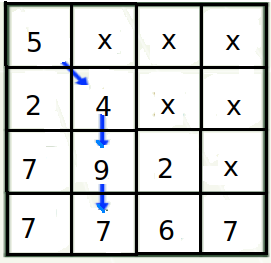
\includegraphics[width=100pt,height=100pt]{slike/dp-table-1.png}
		\caption{Primjer putanje pijuna. Ukupna težina označenog puta je 25.} \label{fig:pijun-putanja}
	\end{figure}

Memoizaciju izvršavamo matricom $M$: na polju $(i , j)$ pamtimo
vrijednost najboljeg puta od pozicije $(0, 0)$ (gornji lijevi ugao) do pozicije $(i , j)$. Pokušajmo   rekurzivno odrediti vrijednost $A(i,j)$ u zavisnosti od odgovarajućih podproblema. Moguća su dva scenarija, pijun je  došao iz pozicije $(i-1, j-1)$ u poziciju $(i,j)$ ili iz pozicije $(i-1, j)$ u poziciju $(i, j)$. Prema tome, vrijedi rekurzija: 

\begin{equation}
	A(i,j) = \max\{ A(i-1, j-1) + a_{ij}, A(i-1, j) + a_{ij}   \}.
\end{equation}
Bazni slučajevi rekurzije su dati sa 
\begin{equation}
	A(0, 0) = a_{00}, A(0, j) = 0, j > 1.
\end{equation}
Rješenje problema nalazimo sljedećom formulom:
\begin{equation}
	\max_{j=0, \ldots, n-1}A(n-1, j)
\end{equation}

Implementacija ovog rješenje je data sljedećim kodom (pristup odozgo prema dolje).

\begin{minted}{python}
	M = None #matrica sa svim -1
	def init(n):
        
        M = [ [-1] * n for _ in range(n)  ]
		
        M[0][0] = A[0][0] #bazni slučaj
        for j in range(n):
             M[0][j] = 0
	
	def solve(i, j):
		if i == 0:
			return M[0][0]
			
		if M[i][j] != -1: #Podproblem vec izračunat
			return M[i][j]
		
		best = rec(i-1, j)
		if j > 0:
			best = max(best, solve(i-1, j-1))
		M[i][j] = best + A[i, j]
		return M[i][j]

	#instanca
	A= [[4 5 7 0]
    	[2 3 1 3]
    	[1 1 3 1]
    	[2 3 3 3]
        ]	
	init(len(A))
	sum_path = 0
	for j in range(len(A)):
		init(len(A))
		sum_path = max(sum_path, solve(len(A)-1, j))
\end{minted}

\textit{Kompleksnost algoritma}. Rekurzija \texttt{solve} se poziva  $n$ puta. Dalje,  svaki poziv funkcije se izvršava u $O(n^2)$ vremenskoj kompleksnosti. Prema tome, ukupna kompleksnost algoritma je $O(n^3)$.

\end{solution}



\begin{example}
	Rješiti problem ruksaka pomoću dinamičkog programiranja. 
\end{example}

\begin{solution}
	\\
	\textit{Podproblemi}. Riješimo problem ruksaka kapaciteta $j\leq C$ birajući prvih $i\leq n$ proizvoda, tj. one proizvode indekirane sa indeksima $1, \ldots , i$.  Memorišimo rješenje matricom $DP$, konkretno sa $DP[i ][j]$. Dakle, podproblem je definisan parom brojeva $(i,j), i\in \{0, 1, \ldots, n\}, j \in \{0, \ldots, C \}$. 
	
	\textit{Rekurzija}. Posmatrajmo fiksirani podproblem dat parom indeksa $(i, j)$ i nađimo  (manje) podprobleme koji su relevantni za rješavanje njega samog. Vrijedi:
	
	\begin{itemize}
		\item Ako $i$-ti proizvod ne učestvuje u (optimalnom) rješenju podproblema $(i, j)$, tada je $DP[i][j] = DP[i-1][j]  $
		\item     Inače, posmatrajmo podprobleme koji uzimaju u razmatranje prvih $k\in \{1, \ldots, i-1\}$ proizvoda. Prvo, podproblemi kojima je kapacitet veći od $C$ nisu relevantni za rješavanje podproblema $(i,j)$. Posmatrajmo neki podproblem $(k,l), k < i, 0 \leq l < j$. Ako možemo dopustivo dodati $i$-ti proizvod u rješenje ovog podproblema, dobijamo potencijalo rješenje većeg podproblema $(i,j)$. Dakle, ako je $l + w_i \leq j$, potencijalno rješenje podproblema je dato sa vrijednošću $D[k][l] + p_i$.  Prema tome, imamo rekurziju:
	   \begin{align*}
		      DP[i ][j ]& = \max\{ D[i-1][j], \max\{DP[k][j - w_i ] + p_i \mid   \\   & j - w_i \geq  0 \ \wedge\  k=1, \ldots, i-1, j \leq C\}\}.
		\end{align*}
	\end{itemize}
	
	 \textit{ Bazni slučajevi}. Ako je kapacitet ruksaka $C=0$, onda je i cijena takvog rješenja jednaka 0, za sve razmatrane proizvode (u ruksak koji ne može da stane ništa, ne  stavimo proizvode). Dakle, $DP[i][0] = 0.$ Takođe, u ruksak bilo kog kapaciteta $j \leq C$, ukoliko ne postoje proizvodi koji se stavljaju u ruksak, trivijalno ne staju proizvodi, pa je $DP[0][j] = 0, 0 \leq j \leq C$.
	 
	 Rješenje proizvoda se memoriše u strukturi $DP$ na poziciji indeksa $(n, C)$.
	 
	 Implementacija paradigme dinamičkog programiranja za rješavanje problema ruksaka je data narednim k\^odom.
	 
	 \begin{minted}{python}
	 def knapsack(n, C, W, p):
	 	DP = [[0 for x in range(C + 1)] for x in range(n + 1)]
	 
	 	# tabuliranje
	 	for i in range(n + 1):
	 		for j in range(C + 1):
	 			if i == 0 or j == 0:
	 				DP[i][j] = 0
	 			elif W[i-1] <= j:
	 				DP[i][j] = max(p[i-1]
	 				         + DP[i-1][j-W[i-1]],
	 				         DP[i-1][j])
	 			else:
	 				DP[i][j] = DP[i-1][j]
	 
	 	return K[n][C]
	 
	 #instanca:
	 p = [60, 100, 120]
	 W = [10, 20, 30]
	 C = 50
	 n = len(profit)
	 #poziv funkcije
	 print knapSack(n, C, W, p, n)
	 \end{minted}
	 
 \textit{Kompleksnost algoritma}. Najskuplji dio algoritma su dvije ugnježdene \texttt{for} petlje, koje izvršavaju $O(n \cdot C)$ iteracija. Svaka od iteracija se izvršava u konstantnom vremenu, pa je i ukupna kompleksnost algoritma jednaka $O(n \cdot C)$.
\end{solution}

Navedimo primjer jedne instance i $DP$ tabelu koja se kreira rekurzivno. 

Neka je $n = 4$, te neka je kapacitet ruksaka $C= 5$, dok je  $W = (2, 3, 4, 5)$, a $P = (3, 4, 5, 6)$. 
 %https://codecrucks.com/knapsack-problem-using-dynamic-programming/
 U prvom koraku ($i=0$ i $j =0$) se popunjavaju nule u prvoj vrsti i prvoj koloni matrice $DP$, kako je prikazano u sljedećoj tabeli:
  \begin{table}[H]
 	\centering
 	\begin{tabular}{|c|cc|cccccc|}\hline
 
  	$j\rightarrow$     & Proizvod   &              &	 	0	&1&	2	&3	&4	&5 \\ \hline
        
 $i=0$ & 	& 	    & 	        0	&0	&0	&0	&0	&0  \\
 $i=1$ &	$w_1=2$	&$p_1=3$ &	0	& 	& 	& 	& 	&\\ 
 $i=2$ &	$w_2=3$	&$p_2=4$ &	0   &	& 	& 	&	&\\	 
 $i=3$ &	$w_3=4$	&$p_3=5$ &	0	& 	& 	& 	& 	&\\ 
 $i=4$ &	$w_4=5$ &$p_4=6$ &	0	& 	& 	& 	& 	&\\ \hline
 \end{tabular}
\end{table}
 
 Dalje, za $i = 1$, imao sljedeće izračunavanje: 
 \begin{itemize}
 	\item proizvod 1 ima težinu 2 i vrijednost 3, pa u drugoj vrsti matrice $DP$ ($i=1$) sve do trećeg elementa ($j=2$) vrijednosti su 0, dok je krenuvši sa tim elementom, svakoj poziciji dodijeljena vrijednost 3 (=$p_1$). 
 \end{itemize}
Dakle, popunjavamo drugu vrstu kao u sljedećoj tabeli:
 
   \begin{table}[H]
 	\centering
 	\begin{tabular}{|c|cc|cccccc|}\hline
 		
 	$j\rightarrow$	& Proizvod   &              &	 	0	&1&	2	&3	&4	&5 \\ \hline
 		
 		$i=0$ & 	& 	    & 	    0	&0	&0	&0	&0	&0  \\
 		$i=1$ &	$w_1=2$	&$p_1=3$ &	0	&0 	&3 	&3 	&3 	&3\\ 
 		$i=2$ &	$w_2=3$	&$p_2=4$ &	0   &	& 	& 	&	&\\	 
 		$i=3$ &	$w_3=4$	&$p_3=5$ &	0	& 	& 	& 	& 	&\\ 
 		$i=4$ &	$w_4=5$ &$p_4=6$ &	0	& 	& 	& 	& 	&\\ \hline
 	\end{tabular}
 \end{table}
  
  Dalje, za treću vrstu ($i=2$) imamo sljedeću tabelu: 
  
   
  \begin{table}[H]
  	\centering
  	\begin{tabular}{|c|cc|cccccc|}\hline
  		
  		$j\rightarrow$	& Proizvod   &              &	 	0	&1&	2	&3	&4	&5 \\ \hline
  		
  		$i=0$ & 	& 	    & 	    0	&0	&0	&0	&0	&0  \\
  		$i=1$ &	$w_1=2$	&$p_1=3$ &	0	&0 	&3 	&3 	&3 	&3\\ 
  		$i=2$ &	$w_2=3$	&$p_2=4$ &	0   &0	&3 	&4 	&4	&7\\	 
  		$i=3$ &	$w_3=4$	&$p_3=5$ &	0	& 	& 	& 	& 	&\\ 
  		$i=4$ &	$w_4=5$ &$p_4=6$ &	0	& 	& 	& 	& 	&\\ \hline
  	\end{tabular}
  \end{table}
Diskutujmo slučaj $DP[2][4]=4$. Ako rješenje podproblema ne uzima proizvod 2, $DP[1][4]=3$ je potencijalno rješenje. U protivnom, ako se uzme, moguće rješenje razmatranog problema je $4 + DP[2][4-4] = 4 + 0 = 4$. Kako je $\max\{3, 4\}= 4$, slijedi da je $DP[2][4] = 4$.


  Narednom iteracijom, popunjavamo četvrtu vrstu ($i=3$) u prethodnoj tabeli, pa imamo: 

  \begin{table}[H]
	\centering
	\begin{tabular}{|c|cc|cccccc|}\hline
		
		$j\rightarrow$	& Proizvod   &              &	 	0	&1&	2	&3	&4	&5 \\ \hline
		
		$i=0$ & 	& 	    & 	    0	&0	&0	&0	&0	&0  \\
		$i=1$ &	$w_1=2$	&$p_1=3$ &	0	&0 	&3 	&3 	&3 	&3\\ 
		$i=2$ &	$w_2=3$	&$p_2=4$ &	0   &0	&3 	&4 	&4	&7\\	 
		$i=3$ &	$w_3=4$	&$p_3=5$ &	0	&0 	&3 	&4 	&5 	&7 \\ 
		$i=4$ &	$w_4=5$ &$p_4=6$ &	0	& 	& 	& 	& 	&\\ \hline
	\end{tabular}
\end{table}
 Diskutujmo slučaj $DP[3][4]=5$.   Ako rješenje podproblema ne uzima proizvod 3, $DP[2][4]=3 $ je potencijalno rješenje ovog podproblema. Dalje, ako uzima, onda je rješenje $DP[2][4-4] + 5 = 0 + 5 = 5$ potencijalni kandidat za razmatrani podproblem. Kako je $\max\{4, 5\}=5$, slijedi zaključak.
 
   Konačno, posljednjom iteracijom popunjavamo petu vrstu ($i=4$) u prethodnoj tabeli, pa imamo: 
 
 \begin{table}[H]
 	\centering
 	\begin{tabular}{|c|cc|cccccc|}\hline
 		
 		$j\rightarrow$	& Proizvod   &              &	 	0	&1&	2	&3	&4	&5 \\ \hline
 		
 		$i=0$ & 	& 	    & 	    0	&0	&0	&0	&0	&0  \\
 		$i=1$ &	$w_1=2$	&$p_1=3$ &	0	&0 	&3 	&3 	&3 	&3\\ 
 		$i=2$ &	$w_2=3$	&$p_2=4$ &	0   &0	&3 	&4 	&4	&7\\	 
 		$i=3$ &	$w_3=4$	&$p_3=5$ &	0	&0 	&3 	&4 	&5 	&7 \\ 
 		$i=4$ &	$w_4=5$ &$p_4=6$ &	0	&0 	&3 	&4 	&5 	&7\\ \hline
 	\end{tabular}
 \end{table}

 Diskutujmo slučaj $DP[4][5]=7$.  Ako rješenje podproblema ne uzima proizvod 4, $DP[3][5]=7$ je potencijalno rješenje ovog podproblema. Dalje, ako uzima proizvod 4, onda  je i rješenje $DP[4][5-5] + 6 = 0 + 6 = 6$ potencijalni kandidat za razmatrani podproblem. Kako je $\max\{6, 7\}=7$, slijedi zaključak.
 
 \begin{definition}
 	String $s$ je podniz stringa $s_1$ akko se $s$ može dobiti brisanjem
 	karaktera iz stringa $s_1$. \\
 	Npr.  \texttt{acd} je podniz stringa \texttt{abbbcdef}.   
 	
 	Prefiks stringa $s$ dužine $k$ je podstring stringa $s$ koji se sastoji od prvih $k$ karaktera. Npr. prefiks dužine tri stringa \texttt{abbbcdef} je string \texttt{abb}. 
 	
 \end{definition}
 
 \begin{example}
 	\textit{Problem najdužeg zajedničkog podniza} (eng. \textit{the longest common subsequence problem}-- LCSP).  Neka su u ulazu data dva stringa $s_1$ i $s_2$. 
 	
 	Naći najduži mogući string $s$ koji je podniz oba ulazna stringa.  \\
 	
 	Za instancu $s_1=$\texttt{aatdccddc} i $s_2=$\texttt{agccddta}, rješenje je string $s=$\texttt{accdd}. 
 	
 \end{example}

\begin{solution}
	    Definišimo podproblem indukovan parom $(i,j), 0 \leq i \leq |s_1|, 0 \leq j \leq |s_2|$  za dva stringa: prvi predstavlja  prefiks dužine $i$ stringa $s_1$,  a drugi predstavlja prefiks dužine $j$ stringa $s_2$.  Čuvajmo rješenje svakog podproblema indukovanog sa $(i,j)$ u matrici $DP$ na poziciji $(i, j)$, tj. $DP[i][j]$.
	    
	    \textit{Rekurzija}. Neka je dat podproblem $(i, j)$. Nađimo strategiju razbijanja problema na manje podprobleme i sve podprobleme na osnovu kojih se može konstruisati rješenje podproblema $(i, j)$. Posmatrajmo karaktere na pozicijama $i$ i $j$, prvog i drugog ulaznog stringa, redom.  Moguća su dva slučaja.
	    \begin{itemize}
	    	\item $s_1[i-1] = s_2[j-1]$: U ovom slučaju, vrijedi rekurzija $DP[i][j] = 1 + DP[i-1][j-1]$, jer  se optimalno rješenje podproblema $(i-1, j-1)$ tada može proširiti za 1 (karakter $s_1[i-1]$) tako da je novonastalo rješenje optimalno za podproblem $(i,j)$.
	    	\item  $s_1[i-1] \neq s_2[j-1]$: U ovom slučaju, sigurno karkter predstavljen parom karaktera $(s_1[i-1]$, $s_2[j-1])$ ne doprinosi optimalnom rješenju podproblema $(i,j)$. Dakle,  za određivanje optimuma podproblema $(i,j)$ relevantna su dva podproblema: $(i-1, j)$ i $(i, j-1)$, nastala izbacivanjem krajnjih karaktera prvo u prvom, pa onda u drugom prefiksu. Duže rješenja ta dva podproblema će činiti i optimalno rješenje za podproblem $(i,j)$. Dakle, u ovom slučaju vrijedi rekurzija:
	    	$$DP[i][j] = \max \{ DP[i-1][j], DP[i][j-1] \} $$ 
	    	
	    \end{itemize}
	    Rješenje problema nalazimo u $DP$ na poziciji $(|s_1|, |s_2|)$. 
	    
	    \textit{Bazni slučajevi}. Ako je jedan od ulaznih strigova prazan, rješenje je jednako 0, tj.  $DPi][0]= 0, 0 \leq i \leq |s_1|,  DP[0][j] = 0, 0 \leq j \leq |s_2|$. 
	    
	 Implementacija paradigme dinamičkog programiranja za rješavanje LCSP je data narednim k\^odom. 
 \begin{minted}{python}
	    	
	    	def LCS(s1, s2):
	    	      
	    	  if len(s1)==0 or len(s2)==0:
	    	     return 0
	    	     
	    	  DP = [ [0]*(len(s2)+1) for _ in range(len(s1)+1)]
	              for i in range(1, len(s1)+1):
	    	      for j in range(1, len(s2)+1):
	    		     if s1[i] == s2[i]: 
	    		         DP[i][j] = DP[i-1][j-1] + 1:
	    		     else:
	    		         DP[i][j] = max(DP[i-1][j], DP[i][j-1])
	    		          
	    	return DP[len(s1)][len(s2)]        
	    		           
	    	      
	    	#instanca:
	    	s1 = "abcdcdcdaa"
	    	s2 = "abbaabcccddd"
	    	lcs = LCS(s1, s2)
	    	print("Duzina LCS-a je: ", lcs)     
 \end{minted}
	     Primijetimo da implementacija koristi princip odozdo-nagore.
	     
	     \textit{Kompleksnost algoritma}. Dvije \texttt{for}-petlje  izvršavaju ukupno $O(|s_1|\cdot |s_2|)$ iteracija. Svaka od iteracija se izvršava u konstantnom vremenu, pa je shodno tome ukupno vrijeme izvršavanja algoritma jednako $O(|s_1| \cdot |s_2|)$. Ako je $n = \max\{|s1|, |s2|\}$, dobijamo kvadratnu $O(n^2)$ kompleksnost. 
	     
	     \begin{figure}[H]
	     	\centering
	     	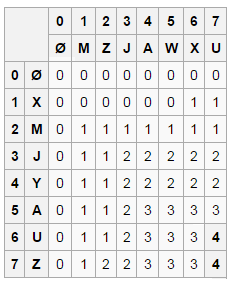
\includegraphics[width=100pt,height=100pt]{slike/dp-lcs-table.png}
	     	\caption{DP matrica za dva stringa $s_1=$\texttt{MZJAWXU} i $s_2=$\texttt{XMJYAUZ}. Rješenje je dužine 4 (pogledati donji desni ugao matrice). }
	     \end{figure}
 	      
\end{solution}

%https://www.programiz.com/dsa/longest-common-subsequence ==> primjer tabele sa rješenjem...

\begin{example}
	\textbf{\textit{Problem sume podskupa}}. Neka je u ulazu dat niz \emph{niz} (od $n$) nenegativnih cijelih brojeva i broj \textit{sum}. 
	
	Da li postoji podniz datog niza \emph{niz} čija je suma elemenata
	  jednaka vrijednosti  \textit{sum}.
\end{example}

\begin{solution}
   Definišimo podproblem indukovan parom $(i, j)$, $0 \leq i \leq n, 0 \leq j \leq sum$ koji razmatra prvih $i$ brojeva niza \emph{niz} i za njih vraća odgovor ($True$ ili $False$) da li se među njima nalaze brojevi čiji je zbir jednak \emph{j}. Čuvajmo rješenje ovakvog podproblema u matrici $DP$, na poziciji $(i,j)$, tj. $DP[i][j]$. 
   
   \textit{Rekurzija}. Analizirajmo podprobleme koji su relevantni za rješavanje podproblema $(i,j)$. Razlikujemo dva slučaja:
   \begin{itemize}
   	\item $i$-ti element niza \emph{niz} može biti dio rješenja. Tada se podproblem $(i, j)$ redukuje na podproblem $(i-1, j-niz[i-1])$ -- pod uslovom da je  $j-niz[i-1]\geq  0$ --  i podproblem $(i-1, j)$
   	    $$ DP[i, j] = DP[i-1, j]\ \vee\  DP[i-1][ j- niz[i-1] ]. $$
   	\item $i$-ti element niza \emph{niz} nije dio rješenja. Tada se podproblem $(i, j)$ redukuje na podproblem $(i-1, j)$, a rekurzija data sa 
   	$$ DP[i][j] = DP[i-1][j]. $$

   \end{itemize}
   
   \textit{Bazni slučajevi}. $DP[i][0] = True, i \geq 0,$ i $DP[0][j] = False,$ za $ j \geq 1$. 
   
    Implementacija paradigme dinamičkog programiranja za rješavanje problema sume podskupa je data narednim k\^odom. 
   
   \begin{minted}{python}
   	  def sum_array(niz, suma):
   	      #tabulation:
   	      DP = [[False] * (suma +1) for _ in range(len(niz) + 1) ]
   	      for i in range(len(niz)+1):
   	          DP[i][0] = True
   	      
   	      for i in range(1, len(niz)+1):   
   	          for j in range(1, suma+1):
   	              if j >= niz[i-1]:
   	                 DP[i][j] = DP[i-1][j-niz[i-1]] or DP[i-1][j]
   	              else:
   	                 DP[i][j] = DP[i-1][j]
   	  
   	  #instanca:
   	  niz = [3, 34, 4, 12, 5, 2]
   	  suma = 9
   	  postoji = sum_array(niz, suma)
   	  print("Postoji podniz sa sumom" if postoji else  
   	        "Ne postoji podniz sa sumom")
   \end{minted}
\end{solution}
Primijetimo da smo dinamičko programiranje implementirali pomoću pristupa \textit{odozdo prema gore}. 

Implementirajmo sada dinamičko programiranje za ovaj problem pristupom odozgo prema dolje.

   \begin{minted}{python}
	def init(niz, sum):
		global DP
		DP = [[-1] * (sum +1) for _ in range(len(niz) + 1) ]
	
	
	def sum_array_top_down(niz, sum, i, j, DP = [ ]):
	
		if DP[i][j] != -1:
			return DP[i][j]
	
		if j == 0:
			DP[i][0] = True
			return True 
		if i == 0: 
			DP[0][j] == False
			return False
		#recursion: 
		if j >= niz[i-1]:
			DP[i][j] = sum_array_top_down(niz, sum, i-1, j, DP) 
	                or sum_array_top_down(niz, sum, i, j-niz[i-1], DP)
			return DP[i][j]
		else:
			DP[i][j] = sum_array_top_down(niz, sum, i-1, j, DP)
			return DP[i][j]
\end{minted}  

\textit{Kompleksnost algoritma}. Broj iteracija koje se izvršavaju je jednak $O(n \cdot sum)$. Svaka iteracija se izvršava u konstantnom vremenu, pa je i ukupna kompleksnost algoritma jednaka  $O(n \cdot sum)$. Dakle, ako je vrijednost \emph{sum} ogromna, ekponencijalno velika u odnosu na veličinu niza, ovakav algoritam će biti neefikasan. 



\begin{example}
	\textbf{\textit{Problem rezanja štapa}}. Dat je štap dužine $n$ i lista \textit{price} koja odgovara cijenama štapa dužine $i$, za sve $1 \leq i \leq n$.
	
	Pronaći optimalan način da se isiječe  štap na manje
	štapove da bi se maksimizovao ukupan profit.
\end{example}


\begin{solution}
	Posmatrajmo primjer jedne instance problema: 
	$$ price = [1, 5, 8, 9, 10,
	17, 17, 20].$$  Neka je štap dužine $d=4$.
	Rješenje konkretne instance je rezati štap na dva dijela dužine od po 2. Zarada je u tom slučaju jednaka $5 + 5 = 10$. 
	
	 Podprobleme datog problema indukujemo indeksima $i$, $0 \leq i \leq n$, gdje vrijednost indeksa $i$ označava instancu problem rezanja štapa dužine $i$. Pretpostavimo da vrijednost optimalnog rezanja (tj. optimalno rješenje)  instance dužine $i$ čuvamo u nizovnoj strukturi $DP$ na poziciji $i$, tj. $DP[i]$.
	 
	 \textit{Rekurzija}. Podproblem indukovan vrijednošću $i$ možemo  riješiti rješavajući podprobleme koji su indukovani sa $k$, $0 \leq k < i$. To znači da štap dužine $i$ dijelimo na dva dijela, dužine $k$ (sa cijenom $price[k-1]$) $i$ štap dužine $(i-k)$, koji opet razmatramo rekurzivno.  
	 
	 Rekurzija u ovom slučaju izgleda ovako:
	 
	 $$ DP[i] = \max \{ DP[i-k] + price[k-1] \mid 1 \leq k \leq i\}.$$
	 
	 Za bazne slučajeve je $DP[0] = 0$, dok je $DP[1] = price[0]$.
	 Rješenje inicijalnog problema se nalazi u $DP[n]$.
\end{solution}

 Implementacija paradigme dinamičkog programiranja za rješavanje problema  rezanja štapa je data narednim k\^odom. 
 
 \begin{minted}{python}
	def stick_cut(d, price):

		DP = [-1] * (d+1)  #init
		DP[0] = 0
		DP[1] = price[0]

		for i in range(2, d+1):
			for k in range(1, i+1):
				if DP[i] < DP[i-k] + price[k-1]: 
					DP[i] =  DP[i-k] + price[k-1]
		return DP[d]       
     
     #instanca
     d = 4
     price = [1, 5, 8, 9, 10, 17, 17, 20] 
     max_profit = stick_cut(d, price)      #poziv:
     print(max_profit)
 \end{minted}

\textit{Kompleksnost algoritma}. Dvije \texttt{for} petlje izvršavaju ukupno najviše $O(d^2)$. Kako se svaka iteracija izvršava u konstantnom vremenu, zaključujemo da je kompleksnost algoritma jednaka $O(d^2)$.

\textit{Napomena}. Pogledajmo drvo koje se kreira algoritmom grube sile na slici~\ref{fig:brute-force-stick-cut}  pri rješavanju problema rezanja štapa za $d=4$. Ovaj pristup enumeriše sva moguća rješenja za rezanje štapa dužine $d=4$. Prvo uzima cio štap u razmatranje (i njegovu cijenu), zatim otkida dio štapa dužine 1, dok se ostatak štapa (dužine 3) rješava (dijeli) rekurzivno itd. Kompletno rješenje dobijamo sa listovima stabla (označeni sa 0). 
\begin{center}
	\begin{figure}[H]
		\centering
		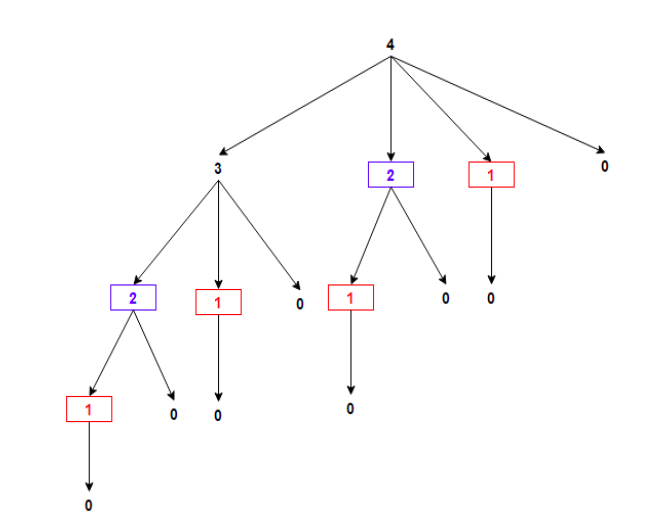
\includegraphics[width=270pt,height=220pt]{slike/brute-force-cutting-stick.png}
		
		\caption{Drvo grananja paradigme grube sile za rješavanje problema rezanja štapa.}\label{fig:brute-force-stick-cut}
	\end{figure}
\end{center}



  Npr. put koji posjećuje čvorove sa oznakama 4 $\rightarrow$ 3 $\rightarrow$ 2 $\rightarrow$ 1 $\rightarrow$ 0, odgovara rješenju u kojem se štap sječe na 4 manja štapa dužine 1 (cijene $4 \times price[0]$). Slično, za put koji posjećuje čvorove sa oznakama 4 $\rightarrow$ 3 $\rightarrow$ 1 $\rightarrow$ 0, odgovara rješenju u kojem se štap sječe na dva manja štapa dužine 1, te jedan dužine 2 (cijene $2 \times price[0] + price[1]$).   
  
   Jasno se vidi da se podproblemi isprepliću, tj. da se, npr. rješavanje problema štapa dužine dva računa više (dva) puta. U slučaju dinamičkog programiranja implementiran  pristupom odozgo prema dolje, stablo će biti značajno redukovano, jer neće postojati rekalkulacije istih podproblema (dakle, nema identičnih kopija podstabala u različitim regionima DP stabla). 
 

\section*{Zadaci}

\begin{enumerate}
	\item Riješiti problem trgovačkog putnika pomoću algoritamske paradigme grube sile.
	\item Riješiti problem ruksaka pomoću algoritamske paradigme grube sile.
	\item Dati  su brojevi  $0 \leq  M  <  N  \leq  1,000,000$. Odrediti  najmanji  broj  sastavljen  samo  od 
	neparnih cifara, koji pri dijeljenju sa $N$ daje ostatak $M$. Ukoliko traženi broj ne postoji, vratiti $−1$. 
	
	 \item Neka su dati prirodni brojevi $n$, koji označava broj promjenljivih, i $s$, koji označava sumu promjenljivih. Uz
pomoć rekurzivnih algoritama napisati program koji pronalazi sva moguća rješenja
za promjenljive  kojih ima $n$ i  čija   suma treba biti jednaka $ s$. 

\textit{Instanca}. $n = 5, s = 4$;
\textit{Rješenje}. 70. \\
\textit{Napomena}:
instanca predstavlja jednačinu $x_1 + x_2 + x_3 + x_4 + x_5 = 4, x_i \in \mathbb{N}$. 
Sva moguća rješenja su:
$(1\ 1\ 1\ 1\ 0), (1\ 0\ 1\ 1\ 1), (0\ 1\ 1\ 1\ 1), \ldots ,$ $(2\ 1\ 0\ 0\ 1), \ldots , (2\ 2\ 0\ 0\ 0)$ itd.
	%pohlepni algoritmi (dva zadatka) 
	%https://www.geeksforgeeks.org/minimum-product-subset-array/
	\item Pronaći podskup elemenata niza tako da je proizvod elemenata u podskupu minimalan. Koristiti paradigmu pohlepnih algoritama.\\
	 \textit{Instanca}. $niz = [ -1, -1, -2, 4, 3]$; \textit{Rješenje}.  -24 ($=(-2 )\cdot (-1) \cdot (-1) \cdot 4 \cdot 3$). 
	
	%https://www.geeksforgeeks.org/greedy-algorithm-egyptian-fraction/
	\item Svaki pozitivan razlomak možemo predstaviti predstaviti kao zbir jedinstvenih jediničnih razlomaka. Razlomak je jedinični razlomak ako je brojnik 1, a nazivnik pozitivan cijeli broj; npr. $1/3$ je jedinični razlomak. Npr. $2/3= 1/2 + 1/6, 3/7=1/3 + 1/11 + 1/231.$   Uz pomoć paradigme pohlepnih algoritama, za proizvoljan razlomak, naći jedinične razlomke koje u zbiru daju taj razlomak.  
	
	
	\item Riješiti problem nalaska najdužeg zajedničkog podniza dva stringa pomoću dinamičkog programiranja pristupom odozgo prema dolje. 
	
	\item Neka je dat niz brojeva u ulazu. Konstruisati algoritam dinamičkog programiranja koji daje odgovor na pitanje li postoji particionisanje niza na dva (disjunktna) skupa tako da je zbir u obe particije jednak.
	\item Implementirati metod dinamičkog progrmairanja  za problem rezanja štapa koristeći pristup odozgo prema dolje.
	
	\item Neka su u ulazu data dva striga $s_1$ i $s_2$. Uz pomoć dinamičkog programiranja, pronaći najkraći string $s$ tako da
	su stringovi $s_1$ i $s_2$ podnizovi stringa $s$.
	\item  Data  je riječ i riječnik (skup riječi). Ispitati da li se riječ može podijeliti na segmente (podstringove) tako da oni pripadaju riječniku. \\
	
	\textit{Instanca}. $$dict = \{\texttt{this}, \texttt{th}, \texttt{is}, \texttt{famous}, \texttt{Word}, \texttt{break}, \texttt{b}, \texttt{r}, \texttt{e}, \texttt{a}, \texttt{k},	\texttt{br}, \texttt{bre}, \texttt{brea}, \texttt{ak}, \texttt{problem} \} $$ te   $$word = \texttt{Wordbreakproblem}.$$  
	\textit{Rješenje}. \texttt{Word break problem},  kao jedno od rješenja.
	
	\item Neka je dat pravougaonik dimenzija $N\times M$. Pretpostavimo da imamo na raspolaganju beskonačan broj pločica
	formata $2^i \times 2^i$, $i = 0, 1, 2, 3, \ldots $. 
	
	Napisati program koji rekurzivno pronalazi minimalan broj pločica koji je potreban da bi se
	popločao pravougaonik datih dimenzija.
	
	\textit{Instanca}.  $N = 6, M=5$;	\textit{Rješenje}. 9 (pločica) -- vidjeti narednu sliku. %~\ref{fig:plocice}. 
	
	\begin{figure}[H]
	    \centering
		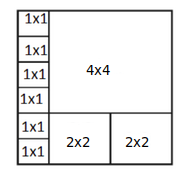
\includegraphics[width=120pt,height=100pt]{slike/plococe-dp-zadatak.png}
		\label{fig:plocice}
		\caption{Optimalno pokrivanje ploče 6 $\times$ 5}
	\end{figure}

\item Napisati program koji generiše sve mogućnosti da se stavi $+$ ili $-$ ili ništa između brojeva $1,2,\ldots,9$ (ovim redom) tako da se kao rezultat izvršenja operacija dobije vrijednost 100. Npr. jedno takvo rješenje je $1 + 2 + 3 - 4 + 5 + 6 + 78 + 9 = 100$.
 
 \item Za dva stringa, napisati program koji ispisuje najkraći niz umetanja i brisanja karaktera u prvi string čijom se primjenom  dobija drugi string.
\end{enumerate}